 %% Copyright (C) 2011, Andrea Cimino, All Rights Reserved.
 %% This file is distributed under the terms of the Creative Commons
 %% Licence Non-Commercial Share-Alike license


%%%% 12 Aprile
%% Useful stuff for separate compilation.
\ifx\ismaindoc\undefined
\providecommand{\inbpdocument}{
 \documentclass[11pt,a4paper,twoside,titlepage]{scrbook}
%%%%%%%%%%%%%%%%%%%%%%%%%%%%%%%%
%%%%%%%%%%% PACKAGES %%%%%%%%%%%
%%%%%%%%%%%%%%%%%%%%%%%%%%%%%%%%
% encoding
\usepackage[utf8x]{inputenc}
\usepackage[italian]{babel} % babel (suddivisione parole in sillabe)

\usepackage{amsfonts} % matematica
\usepackage{amsmath} % matematica
\usepackage{amssymb} % simboli vari
\usepackage{calrsfs}
\usepackage{caption}
\usepackage{enumerate}
\usepackage{extarrows} % matematica
\usepackage{keyval}
\usepackage{manfnt} % Simboli curva
\usepackage{mathtools} % matematica
\usepackage{multirow} 
\usepackage[usenames, dvipsnames]{color} % colori con nome
\usepackage[pdftex]{graphicx}
\usepackage{epstopdf} % gestione file EPS
\usepackage{wrapfig} % per figure circondate da testo
\usepackage{framed}	% teoremi framed
\usepackage{fancyhdr} % header buffi
\usepackage[T1]{fontenc} % gestione hbox e vbox
\usepackage[a4paper]{geometry}
\usepackage{microtype} % gestione hbox e vbox
\usepackage[thref, amsthm, amsmath, framed, hyperref]{ntheorem} % teoremi (avanzata)
%% \usepackage{prooftree} % gestione prof-tree
\usepackage{rotating}
\usepackage{stmaryrd}
\usepackage{subfig}
\usepackage{syntax} % syntattic stuff
\usepackage{txfonts}
\usepackage{verbatim} % migliorie al verbatim
%\usepackage{hyperref}
%% \usepackage{qtree}
\usepackage{fancyvrb}
\usepackage{listings}
\usepackage{cancel}
\usepackage{tikz}

\usepackage{bbding} %% Icons

%%%%%%%%%%%%%%%%%%%%%%%%%%%%%%%%
%%%%%%%%%%% GEOMETRY %%%%%%%%%%%
%%%%%%%%%%%%%%%%%%%%%%%%%%%%%%%%
\geometry{verbose,tmargin=2cm,bmargin=2.5cm,lmargin=2.5cm,rmargin=2cm}
\parindent0ex %% Remove paragraph indenting

%%%%%%%%%%%%%%%%%%%%%%%%%%%%%%%%
%%%%%%%%%%% CODE ENV %%%%%%%%%%%
%%%%%%%%%%%%%%%%%%%%%%%%%%%%%%%%
% codice
\newcounter{count}
\setcounter{count}{0}
\newenvironment{code}[1]
{
\color{lightgray}\hrulefill\color{code}
\stepcounter{count} {\bf\small Listato di codice \arabic{count}: {#1} }
\verbatim
}
{
\endverbatim
\color{lightgray}\hrulefill
\color{black}
\\
}

% codice semplice
\newenvironment{simplecode}
{
\color{code} \tt
}
{
\rm
}

 % Notation issues

%% Proof trees.
%\input prooftree
\newcommand*{\nohyp}{\phantom{x}}

%% C++.
\newcommand*{\Cplusplus}{{C\nolinebreak[4]\hspace{-.05em}\raisebox{.4ex}
{\tiny\bf ++}}}

%% BNF rules.
\newcommand*{\vbar}{\mathrel{\mid}}

%% Abstract syntax of the analyzed language.
\newcommand*{\Type}{\mathrm{Type}}
\newcommand*{\dType}{\mathrm{dType}}
\newcommand*{\dT}{\mathrm{dT}}
\newcommand*{\sType}{\mathrm{sType}}
\newcommand*{\sT}{\mathrm{sT}}
\newcommand*{\cType}{\mathrm{cType}}
\newcommand*{\cT}{\mathrm{cT}}
\newcommand*{\Integer}{\mathrm{Integer}}
\newcommand*{\Bool}{\mathrm{Bool}}
\newcommand*{\Id}{\mathrm{Id}}
\newcommand*{\id}{\mathrm{id}}
\newcommand*{\rId}{\mathrm{rId}}
\newcommand*{\idx}{\mathrm{x}}
\newcommand*{\ridx}{\underline{\mathrm{x}}}
\newcommand*{\Exp}{\mathrm{Exp}}
\newcommand*{\Exps}{\mathrm{Exps}}
\newcommand*{\Decl}{\mathrm{Decl}}
\newcommand*{\exceptDecl}{\mathrm{exceptDecl}}
\newcommand*{\Catch}{\mathrm{Catch}}
\newcommand*{\Stmt}{\mathrm{Stmt}}
\newcommand*{\Label}{\mathrm{Label}}
\newcommand*{\Con}{\mathrm{Con}}
\newcommand*{\con}{\mathrm{con}}
\newcommand*{\fps}{\mathrm{fps}}
\newcommand*{\funBody}{\mathrm{Body}}
\newcommand*{\funbody}{\mathrm{body}}
\newcommand*{\main}{\mathrm{main}}
\newcommand*{\es}{\mathrm{es}}
\newcommand*{\formParams}{\mathrm{formParams}}
\newcommand*{\emptysequence}{\boxempty}
\newcommand*{\Glob}{\mathrm{Glob}}

%% Sets of configurations
\newcommand*{\NTe}{\Gamma_\mathrm{e}}
\newcommand*{\NTb}{\Gamma_\mathrm{b}}
\newcommand*{\NTd}{\Gamma_\mathrm{d}}
\newcommand*{\NTg}{\Gamma_\mathrm{g}}
\newcommand*{\NTs}{\Gamma_\mathrm{s}}
\newcommand*{\NTk}{\Gamma_\mathrm{k}}
\newcommand*{\Te}{T_\mathrm{e}}
\newcommand*{\Tb}{T_\mathrm{b}}
\newcommand*{\Td}{T_\mathrm{d}}
\newcommand*{\Tg}{T_\mathrm{g}}
\newcommand*{\Ts}{T_\mathrm{s}}
\newcommand*{\Tk}{T_\mathrm{k}}

%% Lambda notation.
\newcommand*{\lambdaop}{\mathop{\lambda}\nolimits}

%% Sets of (no better specified) configurations.
\newcommand*{\NT}[1]{\Gamma_{#1}}
\newcommand*{\NTq}{\Gamma_q}
\newcommand*{\Tq}{T_q}

%% Denotable values.
\newcommand*{\dVal}{\mathrm{dVal}}
%% Storeable values.
\newcommand*{\sVal}{\mathrm{sVal}}
\newcommand*{\sval}{\mathrm{sval}}

%% Control modes.
\newcommand*{\CtrlMode}{\mathord{\mathrm{CtrlMode}}}
\newcommand*{\cm}{\mathrm{cm}}
%% Branch modes.
%\newcommand*{\BranchMode}{\mathord{\mathrm{BranchMode}}}
\newcommand*{\GotoMode}{\mathord{\mathrm{GotoMode}}}
\newcommand*{\SwitchMode}{\mathord{\mathrm{SwitchMode}}}
\newcommand*{\cmgoto}{\mathop{\mathrm{goto}}\nolimits}
\newcommand*{\cmswitch}{\mathop{\mathrm{switch}}\nolimits}
\newcommand*{\cmbreak}{\mathop{\mathrm{break}}\nolimits}
\newcommand*{\cmcontinue}{\mathop{\mathrm{continue}}\nolimits}
\newcommand*{\cmreturn}{\mathop{\mathrm{return}}\nolimits}
%% Exec mode.
\newcommand*{\cmexec}{\mathrm{exec}}
%% Value mode.
\newcommand*{\ValMode}{\mathord{\mathrm{ValMode}}}
\newcommand*{\cmvalue}{\mathop{\mathrm{value}}\nolimits}
%% Environment mode.
\newcommand*{\EnvMode}{\mathord{\mathrm{EnvMode}}}
\newcommand*{\cmenv}{\mathrm{env}}
%% Exception modes.
\newcommand*{\ExceptMode}{\mathord{\mathrm{ExceptMode}}}
\newcommand*{\cmexcept}{\mathrm{except}}

%% Control states.
\newcommand*{\CtrlState}{\mathord{\mathrm{CtrlState}}}
\newcommand*{\cs}{\mathord{\mathrm{cs}}}
%% Value states.
\newcommand*{\ValState}{\mathord{\mathrm{ValState}}}
\newcommand*{\valstate}{\upsilon}
%% Environment states.
%\newcommand*{\EnvState}{\mathord{\mathrm{EnvState}}}
%% Exception states.
\newcommand*{\ExceptState}{\mathord{\mathrm{ExceptState}}}
\newcommand*{\exceptstate}{\varepsilon}

%% Keywords.
\newcommand*{\kw}[1]{\mathop{\textup{\textbf{#1}}}}

\newcommand*{\bop}{\mathbin{\mathrm{bop}}}
%\newcommand*{\uop}{\mathop{\mathrm{uop}}}

%% Things that hold by definition.
\newcommand{\defrel}[1]{\mathrel{\buildrel \mathrm{def} \over {#1}}}
\newcommand{\defeq}{\defrel{=}}
\newcommand{\defiff}{\defrel{\Longleftrightarrow}}
%\newcommand{\defeq}{=}
%\newcommand{\defiff}{\Longleftrightarrow}

%% Divergence relation
\newcommand{\diverges}{\,\mathord{\buildrel \infty \over \longrightarrow}}

%% Special letters denoting sets and algebras.
\providecommand*{\Nset}{\mathbb{N}}             % Naturals
\providecommand*{\Qset}{\mathbb{Q}}             % Rationals
\providecommand*{\Zset}{\mathbb{Z}}             % Integers
\providecommand*{\Rset}{\mathbb{R}}             % Reals

%% Calligraphic alphabet.
\newcommand*{\calA}{\ensuremath{\mathcal{A}}}
\newcommand*{\calB}{\ensuremath{\mathcal{B}}}
\newcommand*{\calC}{\ensuremath{\mathcal{C}}}
\newcommand*{\calD}{\ensuremath{\mathcal{D}}}
\newcommand*{\calE}{\ensuremath{\mathcal{E}}}
\newcommand*{\calF}{\ensuremath{\mathcal{F}}}
\newcommand*{\calG}{\ensuremath{\mathcal{G}}}
\newcommand*{\calH}{\ensuremath{\mathcal{H}}}
\newcommand*{\calI}{\ensuremath{\mathcal{I}}}
\newcommand*{\calJ}{\ensuremath{\mathcal{J}}}
\newcommand*{\calK}{\ensuremath{\mathcal{K}}}
\newcommand*{\calL}{\ensuremath{\mathcal{L}}}
\newcommand*{\calM}{\ensuremath{\mathcal{M}}}
\newcommand*{\calN}{\ensuremath{\mathcal{N}}}
\newcommand*{\calO}{\ensuremath{\mathcal{O}}}
\newcommand*{\calP}{\ensuremath{\mathcal{P}}}
\newcommand*{\calQ}{\ensuremath{\mathcal{Q}}}
\newcommand*{\calR}{\ensuremath{\mathcal{R}}}
\newcommand*{\calS}{\ensuremath{\mathcal{S}}}
\newcommand*{\calT}{\ensuremath{\mathcal{T}}}
\newcommand*{\calU}{\ensuremath{\mathcal{U}}}
\newcommand*{\calV}{\ensuremath{\mathcal{V}}}
\newcommand*{\calW}{\ensuremath{\mathcal{W}}}
\newcommand*{\calX}{\ensuremath{\mathcal{X}}}
\newcommand*{\calY}{\ensuremath{\mathcal{Y}}}
\newcommand*{\calZ}{\ensuremath{\mathcal{Z}}}

%% Declarators for functions and relations.
\newcommand*{\reld}[3]{\mathord{#1}\subseteq#2\times#3}
\newcommand*{\fund}[3]{\mathord{#1}\colon#2\to#3}
\newcommand*{\pard}[3]{\mathord{#1}\colon#2\rightarrowtail#3}

%% Logical quantifiers stuff.
\newcommand{\st}{\mathrel{.}}
\newcommand{\itc}{\mathrel{:}}

%% Domain, codomain and range of a function.
\newcommand*{\dom}{\mathop{\mathrm{dom}}\nolimits}
%\newcommand*{\cod}{\mathop{\mathrm{cod}}\nolimits}
%\newcommand*{\range}{\mathop{\mathrm{range}}\nolimits}

%% Restriction of a function.
\newcommand*{\restrict}[1]{\mathop{\mid}\nolimits_{#1}}

%% Type of a constant.
\newcommand*{\type}{\mathop{\mathrm{type}}\nolimits}

%% Lubs, glbs, and fixed points.
\newcommand*{\lub}{\mathop{\mathrm{lub}}\nolimits}
%\newcommand*{\glb}{\mathop{\mathrm{glb}}\nolimits}
\newcommand*{\lfp}{\mathop{\mathrm{lfp}}\nolimits}
\newcommand*{\gfp}{\mathop{\mathrm{gfp}}\nolimits}

%% Generic widening.
\newcommand*{\widen}{\mathbin{\nabla}}

%% Set theory.
\renewcommand{\emptyset}{\varnothing}

%\newcommand*{\wpc}{\mathop{\wp_\mathrm{c}}\nolimits}
%\newcommand*{\wpf}{\mathop{\wp_\mathrm{f}}\nolimits}
%\newcommand*{\wpn}{\mathop{\wp_\mathrm{n}}\nolimits}

\newcommand*{\sseq}{\subseteq}
\newcommand*{\sseqf}{\mathrel{\subseteq_\mathrm{f}}}
\newcommand*{\sslt}{\subset}
%\newcommand*{\Sseq}{\supseteq}
%\newcommand*{\Ssgt}{\supset}

%\newcommand{\Nsseq}{\nsubseteq}

\newcommand*{\union}{\cup}
\newcommand*{\bigunion}{\bigcup}
%\newcommand*{\biginters}{\bigcap}
\newcommand*{\inters}{\cap}
\newcommand*{\setdiff}{\setminus}

\newcommand{\sset}[2]{{\renewcommand{\arraystretch}{1.2}
                      \left\{\,#1 \,\left|\,
                               \begin{array}{@{}l@{}}#2\end{array}
                      \right.   \,\right\}}}

%% Base sets.
\newcommand*{\ttv}{\mathrm{tt}}
\newcommand*{\ffv}{\mathrm{ff}}
\newcommand*{\divop}{\mathbin{/}}
\newcommand*{\modop}{\mathbin{\%}}
\newcommand*{\andop}{\mathbin{\textbf{\textup{and}}}}
\newcommand*{\orop}{\mathbin{\textbf{\textup{or}}}}
\newcommand*{\notop}{\mathop{\textbf{\textup{not}}}}

\newcommand*{\FI}{\mathop{\mathrm{FI}}\nolimits}
\newcommand*{\DI}{\mathop{\mathrm{DI}}\nolimits}
\newcommand*{\SL}{\mathop{\mathrm{SL}}\nolimits}
%\newcommand*{\match}{\mathop{\mathrm{match}}\nolimits}

\newcommand*{\Env}{\mathord{\mathrm{Env}}}
\newcommand*{\emptystring}{\mathord{\epsilon}}

%% Exceptions.
\newcommand*{\RTSExcept}{\mathord{\mathrm{RTSExcept}}}
\newcommand*{\rtsexcept}{\chi}
\newcommand*{\Except}{\mathord{\mathrm{Except}}}
\newcommand*{\except}{\xi}
\newcommand*{\none}{\mathtt{none}}
\newcommand*{\divbyzero}{\mathtt{divbyzero}}
\newcommand*{\stkovflw}{\mathtt{stkovflw}}
\newcommand*{\datovflw}{\mathtt{datovflw}}
\newcommand*{\memerror}{\mathtt{memerror}}
%\newcommand*{\inerror}{\mathtt{inerror}}
%\newcommand*{\nullptr}{\mathtt{nullptr}}
%\newcommand*{\outofboundsptr}{\mathtt{outofboundsptr}}

%% Flags for terminal configurations of catch clauses.
\newcommand*{\caught}{\mathtt{caught}}
\newcommand*{\uncaught}{\mathtt{uncaught}}

%% Static semantics.
\newcommand*{\TEnv}{\mathord{\mathrm{TEnv}}}
\newcommand*{\tinteger}{\mathrm{integer}}
\newcommand*{\tboolean}{\mathrm{boolean}}
\newcommand*{\trtsexcept}{\mathrm{rts\_exception}}

%% Memory structures.
\newcommand*{\Loc}{\mathord{\mathrm{Loc}}}
\newcommand*{\Ind}{\mathrm{Ind}}
\newcommand*{\Addr}{\mathrm{Addr}}
\newcommand*{\Map}{\mathrm{Map}}
%\newcommand*{\eMap}{\mathrm{eMap}}
\newcommand*{\Stack}{\mathord{\mathrm{Stack}}}
\newcommand*{\Mem}{\mathord{\mathrm{Mem}}}
\newcommand*{\stknew}{\mathop{\mathrm{new}_\mathrm{s}}\nolimits}
\newcommand*{\datnew}{\mathop{\mathrm{new}_\mathrm{d}}\nolimits}
\newcommand*{\txtnew}{\mathop{\mathrm{new}_\mathrm{t}}\nolimits}
\newcommand*{\heapnew}{\mathop{\mathrm{new}_\mathrm{h}}\nolimits}
\newcommand*{\heapdel}{\mathop{\mathrm{delete}_\mathrm{h}}\nolimits}
\newcommand*{\datcleanup}{\mathop{\mathrm{cleanup}_\mathrm{d}}\nolimits}
\newcommand*{\smark}{\mathop{\mathrm{mark}_\mathrm{s}}\nolimits}
\newcommand*{\sunmark}{\mathop{\mathrm{unmark}_\mathrm{s}}\nolimits}
\newcommand*{\slink}{\mathop{\mathrm{link}_\mathrm{s}}\nolimits}
\newcommand*{\sunlink}{\mathop{\mathrm{unlink}_\mathrm{s}}\nolimits}
\newcommand*{\asmark}{\mathop{\mathrm{mark}_\mathrm{s}^\sharp}\nolimits}
\newcommand*{\asunmark}{\mathop{\mathrm{unmark}_\mathrm{s}^\sharp}\nolimits}
\newcommand*{\aslink}{\mathop{\mathrm{link}_\mathrm{s}^\sharp}\nolimits}
\newcommand*{\asunlink}{\mathop{\mathrm{unlink}_\mathrm{s}^\sharp}\nolimits}
\newcommand*{\aswiden}{\mathop{\mathrm{widen}}\nolimits}
\newcommand*{\sm}{\dag}
\newcommand*{\fm}{\ddag}
\newcommand*{\topmost}{\mathop{\mathrm{tf}}\nolimits}
%% Short forms of \datcleanup, \sunmark, \sunlink for table.
\newcommand*{\datcleanupshort}{\mathop{\mathrm{cu}_\mathrm{d}}\nolimits}
\newcommand*{\sunmarkshort}{\mathop{\mathrm{um}_\mathrm{s}}\nolimits}
\newcommand*{\sunlinkshort}{\mathop{\mathrm{ul}_\mathrm{s}}\nolimits}

\newcommand*{\location}[1]{\mathord{#1 \; \mathrm{loc}}}
%\newcommand*{\saeval}{\mathop{\mathrm{aeval}}\nolimits}
%\newcommand*{\saupd}{\mathop{\mathrm{aupd}}\nolimits}
\newcommand*{\asupported}{\mathop{\mathrm{supported}^\sharp}\nolimits}
\newcommand*{\aeval}{\mathop{\mathrm{eval}^\sharp}\nolimits}
\newcommand*{\ceval}[1]{\mathop{\mathrm{eval}_{#1}}\nolimits}

%% Abstracts.
\newcommand*{\Abstract}{\mathord{\mathrm{Abstract}}}
\newcommand*{\abs}{\mathord{\mathrm{abs}}}

%% Integer part function.
\newcommand{\intp}{\mathop{\mathrm{int}}\nolimits}

%% Concrete functions and operations.
% Aritmethic
%% \newcommand*{\conadd}{\mathbin{\boxplus}}
%% \newcommand*{\consub}{\mathbin{\boxminus}}
%% \newcommand*{\conmul}{\mathbin{\boxdot}}
%% \newcommand*{\condiv}{\mathbin{\boxslash}}
%% \newcommand*{\conmod}{\mathbin{\boxbar}}
% Boolean
%% \newcommand*{\coneq}{\mathbin{\triangleq}}
%% \newcommand*{\conineq}{\mathbin{\trianglelefteq}}
%% \newcommand*{\conneg}{\mathbin{\daleth}}
%% \newcommand*{\conor}{\mathbin{\triangledown}}
%% \newcommand*{\conand}{\mathbin{\vartriangle}}
\newcommand*{\bneg}{\mathop{\neg}\nolimits}

%% Abstract functions and operations.
% Aritmethic
\newcommand*{\absuminus}{\mathop{\ominus}\nolimits}
\newcommand*{\absadd}{\mathbin{\oplus}}
\newcommand*{\abssub}{\mathbin{\ominus}}
\newcommand*{\absmul}{\mathbin{\odot}}
\newcommand*{\absdiv}{\mathbin{\oslash}}
\newcommand*{\absmod}{\mathbin{\obar}}
% Boolean
\newcommand*{\abseq}{\mathrel{\triangleq}}
\newcommand*{\absneq}{\mathrel{\not\triangleq}}
\newcommand*{\absleq}{\mathrel{\trianglelefteq}}
\newcommand*{\abslt}{\mathrel{\vartriangleleft}}
\newcommand*{\absgeq}{\mathrel{\trianglerighteq}}
\newcommand*{\absgt}{\mathrel{\vartriangleright}}
\newcommand*{\absneg}{\mathrel{\circleddash}}
\newcommand*{\absor}{\mathrel{\ovee}}
\newcommand*{\absand}{\mathrel{\owedge}}

%% Summaries for theorem-like environments
\newcommand{\summary}[1]{\textrm{\textbf{\textup{#1}}}}

%% Filter function extracting the relevant and irrelevant parts.
\newcommand*{\sel}{\mathop{\mathrm{sel}}\nolimits}
\newcommand*{\mem}{\mathop{\mathrm{mem}}\nolimits}

%% Modeling definite exceptions.
%\newcommand*{\None}{\mathrm{None}}

%% Strict Cartesian products.
\newcommand*{\stimes}{\otimes}
\newcommand*{\spair}[2]{{#1} \otimes {#2}}
%\newcommand*{\rstimes}{\rtimes}
%\newcommand*{\rspair}[2]{{#1} \rtimes {#2}}
%\newcommand*{\lstimes}{\ltimes}
%\newcommand*{\lspair}[2]{{#1} \ltimes {#2}}

%% Additional syntax for the numeric type extension supplement
\newcommand*{\iT}{\mathrm{iT}}
\newcommand*{\iType}{\mathrm{iType}}
\newcommand*{\tschar}{\mathrm{signed\_char}}
\newcommand*{\tuchar}{\mathrm{unsigned\_char}}
\newcommand*{\flcon}{\mathrm{fl}}
\newcommand*{\Float}{\mathrm{Float}}
\newcommand*{\sccon}{\mathrm{sc}}
\newcommand*{\sChar}{\mathrm{sChar}}
\newcommand*{\uccon}{\mathrm{uc}}
\newcommand*{\uChar}{\mathrm{uChar}}

%% Additional macros for the extension for extra numeric types
%% Floating point types.
\newcommand*{\tfloat}{\mathrm{float}}
%% Numeric types
\newcommand*{\nType}{\mathrm{nType}}
\newcommand*{\nT}{\mathrm{nT}}

%% Additional macros for the extension to pointer and arrays:
%% Elementary types.
\newcommand*{\eType}{\mathrm{eType}}
\newcommand*{\eT}{\mathrm{eT}}
%% Elementary values.
%\newcommand*{\eValue}{\mathrm{eVal}}
%% Array types.
\newcommand*{\aType}{\mathrm{aType}}
\newcommand*{\aT}{\mathrm{aT}}
%% Record types.
\newcommand*{\rType}{\mathrm{rType}}
\newcommand*{\rT}{\mathrm{rT}}
%% Object types.
\newcommand*{\oType}{\mathrm{oType}}
\newcommand*{\oT}{\mathrm{oT}}
%% Function types.
\newcommand*{\fType}{\mathrm{fType}}
\newcommand*{\fT}{\mathrm{fT}}
%% Memory types.
\newcommand*{\mType}{\mathrm{mType}}
\newcommand*{\mT}{\mathrm{mT}}
%% Pointer types.
\newcommand*{\pType}{\mathrm{pType}}
\newcommand*{\pT}{\mathrm{pT}}
%% Offsets.
\newcommand*{\Offset}{\mathrm{Offset}}
\newcommand*{\nooffset}{\boxempty}
\newcommand*{\indexoffset}[1]{\mathopen{\boldsymbol{[}}{#1}\mathclose{\boldsymbol{]}}}
\newcommand*{\fieldoffset}[1]{\mathop{\boldsymbol{.}}{#1}}
%% Lvalues.
\newcommand*{\lValue}{\mathrm{LValue}}
\newcommand*{\lvalue}{\mathrm{lval}}
%% Rvalues.
\newcommand*{\rValue}{\mathrm{RValue}}
\newcommand*{\rvalue}{\mathrm{rval}}
%%
\newcommand*{\pointer}[1]{{#1}\boldsymbol{\ast}}
\newcommand*{\maddress}[1]{\mathop{\&}{#1}}
\newcommand*{\indirection}[1]{\mathop{\boldsymbol{\ast}}{#1}}
%%
\newcommand*{\locnull}{\mathord{l_\mathrm{null}}}
\newcommand*{\ptrmove}{{\mathop{\mathrm{ptrmove}}\nolimits}}
\newcommand*{\ptrdiff}{{\mathop{\mathrm{ptrdiff}}\nolimits}}
\newcommand*{\ptrcmp}{{\mathop{\mathrm{ptrcmp}}\nolimits}}
%%
\newcommand*{\arraysyntax}[3]{\kw{#1} {#2} \kw{of}\,{#3}}
\newcommand*{\arraytype}[2]{\arraysyntax{array}{#1}{#2}}
\newcommand*{\firstof}{{\mathop{\mathrm{firstof}}\nolimits}}
\newcommand*{\arrayindex}{\mathop{\mathrm{index}}\nolimits}
\newcommand*{\locindex}{\mathop{\mathrm{locindex}}\nolimits}
%%
\newcommand*{\recordsyntax}[3]{\kw{#1} {#2} \kw{of}\,{#3}}
\newcommand*{\recordtype}[2]{\recordsyntax{record}{#1}{#2}}
\newcommand*{\field}{\mathop{\mathrm{field}}\nolimits}
\newcommand*{\locfield}{\mathop{\mathrm{locfield}}\nolimits}
%%
\newcommand*{\NTo}{\Gamma_\mathrm{o}}
\newcommand*{\To}{T_\mathrm{o}}
\newcommand*{\NTl}{\Gamma_\mathrm{l}}
\newcommand*{\Tl}{T_\mathrm{l}}
%\newcommand*{\NTr}{\Gamma_\mathrm{r}}
%\newcommand*{\Tr}{T_\mathrm{r}}
%%
\newcommand*{\arraydatnew}{\mathop{\mathrm{newarray}_\mathrm{d}}\nolimits}
\newcommand*{\arraystknew}{\mathop{\mathrm{newarray}_\mathrm{s}}\nolimits}
\newcommand\Cut{\using\sf cut\thickness.08em\justifies}
\newcommand{\maybeeq}{\mathrel{\buildrel \mathrm{?} \over =}}



\makeatletter
\g@addto@macro\@verbatim\footnotesize
\makeatother



%%%%%%%%%%%%%%%%%%%%%%%%%%%%%%%%
%%%%%%%% THEOREMS FORMAT %%%%%%%
%%%%%%%%%%%%%%%%%%%%%%%%%%%%%%%%
% shaded theorems and proofs command
\definecolor{lightgray}{RGB}{230,230,230}
\def\theoremframecommand{\colorbox{lightgray}}

%%% theorems
\theoremstyle{break}
\theoremheaderfont{\normalfont\bfseries}
\theorembodyfont{\itshape}
\theoremsymbol{\ensuremath{\diamondsuit}}
\theoremseparator{\newline}
\newtheorem{theo}{
\includegraphics[scale=0.11]{imgs/book.png}Teorema}[chapter]

%%% propositions
\theoremstyle{break}
\theoremheaderfont{\normalfont\bfseries}
\theorembodyfont{\itshape}
\theoremsymbol{\ensuremath{\diamondsuit}}
\theoremseparator{\newline}
\newshadedtheorem{proposition}{Proposizione}[chapter]

%%% exercises
\theoremstyle{break}
\theoremheaderfont{\normalfont\bfseries}
\theorembodyfont{\itshape}
\theoremsymbol{\ensuremath{\diamondsuit}}
\theoremseparator{\newline}
\newshadedtheorem{exercise}{Esercizio}[chapter]

%%% propositions
\theoremstyle{break}
\theoremheaderfont{\normalfont\bfseries}
\theorembodyfont{\itshape}
\theoremsymbol{\ensuremath{\diamondsuit}}
\theoremseparator{\newline}
\newshadedtheorem{property}{\PencilRightDown $\; $ Propriet\`a}[chapter]

%%% lemmas
\theoremstyle{break}
\theoremheaderfont{\normalfont\bfseries}
\theorembodyfont{\itshape}
\theoremsymbol{\ensuremath{\diamondsuit}}
\theoremseparator{\newline}
\newshadedtheorem{lemma}[theo]{Lemma}

%%% definitions
\theoremstyle{break}
\theoremsymbol{\ensuremath{\clubsuit}}
\theoremseparator{\newline}
\newshadedtheorem{defn}[theo]{Definizione}

%%% examples
\theoremstyle{break}
\theorembodyfont{\itshape}
\theoremsymbol{\ensuremath{\ast}}
\theoremseparator{\newline}
\newshadedtheorem{example}[theo]{Esempio}

%%% observations
\theoremstyle{break}
\theorembodyfont{\itshape}
\theoremsymbol{\ensuremath{\ast}}
\theoremseparator{\newline}
\newshadedtheorem{observation}[theo]{

\includegraphics[scale=0.06]{imgs/lens.png}
Osservazione
}

%%% notations
\newtheorem*{notaz}{Notazione}

%%% proofs
\newenvironment{thproof}
{
\vskip 0.03cm
\begin{small}
\textit{Dimostrazione. }
\color{code}
}
{
\color{black}
\end{small}
$ \square $
\vskip 0.2cm
}

%Notes
\newenvironment{notes}{%
  \def\FrameCommand{\colorbox{yellow}}%
  \MakeFramed {\FrameRestore}
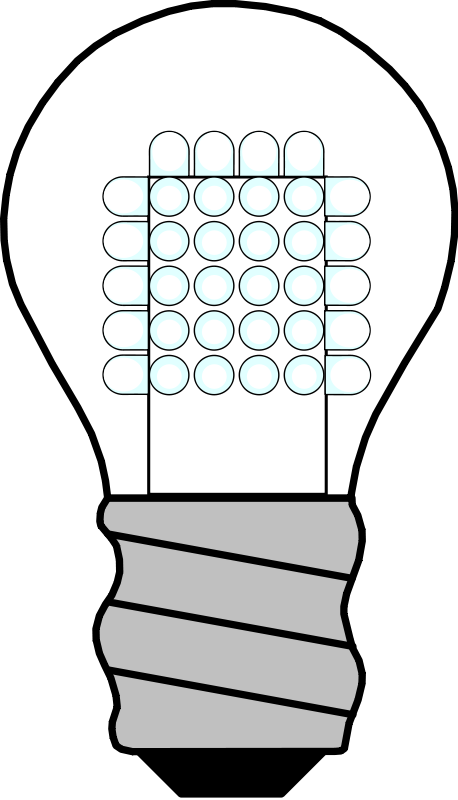
\includegraphics[scale=0.02]{imgs/bulb.png}
 \textbf{Nota} \\
 }%
{\endMakeFramed}

%Work in progress
\newenvironment{workinprogress}{%
  \def\FrameCommand{\colorbox{pink}}%
  \MakeFramed {\FrameRestore}
\lhdbend  \textbf{Work in progress} \\
 }%
{\endMakeFramed}

%Openquestion
\newenvironment{openquestion}{%
  \def\FrameCommand{\colorbox{pink}}%
  \MakeFramed {\FrameRestore}
 \textbf{Domanda aperta} \\
 }%
{\endMakeFramed}

%TODO
\newenvironment{todo}{%
  \def\FrameCommand{\colorbox{pink}}%
  \MakeFramed {\FrameRestore}
 \textbf{TODO} \\
 }%
{\endMakeFramed}

%%%%%%%%%%%%%%%%%%%%%%%%%%%%%%%%
%%%%%%%%%%%% HEADER %%%%%%%%%%%%
%%%%%%%%%%%%%%%%%%%%%%%%%%%%%%%%
\pagestyle{fancy}
% i comandi seguenti impediscono la scrittura in maiuscolo
% dei nomi dei capitoli e dei paragrafi nelle intestazioni
\renewcommand{\chaptermark}[1]{\markboth{#1}{}}
\renewcommand{\sectionmark}[1]{\markright{\thesection\ #1}}
\fancyhf{} % rimuove l'attuale contenuto dell'intestazione
% e del pi\`e di pagina
\fancyhead[LE,RO]{\bfseries\thepage}
\fancyhead[LO]{\bfseries\rightmark}
\fancyhead[RE]{\bfseries\leftmark}
\renewcommand{\headrulewidth}{0.5pt}
\renewcommand{\footrulewidth}{0pt}
\addtolength{\headheight}{0.5pt} % riserva spazio per la linea
\fancypagestyle{plain}{%
\fancyhead{} % ignora, nello stile plain, le intestazioni
\renewcommand{\headrulewidth}{0pt} % e la linea
}


%%%%%%%%%%%%%%%%%%%%%%%%%%%%%%%%
%%%%%%%%%%%% COLORS %%%%%%%%%%%%
%%%%%%%%%%%%%%%%%%%%%%%%%%%%%%%%
\definecolor{code}{gray}{0.3}


%%%%%%%%%%%%%%%%%%%%%%%%%%%%%%%%
%%%%%%%%%%%% NUMBERS %%%%%%%%%%%
%%%%%%%%%%%%%%%%%%%%%%%%%%%%%%%%
\setcounter{tocdepth}{3}
\setcounter{secnumdepth}{3}


%%%%%%%%%%%%%%%%%%%%%%%%%%%%%%%%
%%%%%%%%%%% DOC DATA %%%%%%%%%%%
%%%%%%%%%%%%%%%%%%%%%%%%%%%%%%%%
\title{Appunti di MNO}
\author{Gruppo Informatici Rampanti}
\date{ott 2010 - mag 2011}

\pdfinfo{%
  /Title    (Appunti di MNO)
  /Author   (Andrea Cimino e Lorenzo Muti)
  /Creator  (Andrea Cimino)
  /Producer (Lorenzo Muti)
  /Subject  (MNO)
  /Keywords (MNO)
}


%%%%%%%%%%%%%%%%%%%%%%%%%%%%%%%%
%%%%%%%%%%%%% UTILS %%%%%%%%%%%%
%%%%%%%%%%%%%%%%%%%%%%%%%%%%%%%%
% binary symbols
\newcommand{\modder}{\vdash _{R}}

% vertical gaps
\newcommand{\askip}{\vspace{0.5cm}}
\newcommand{\bskip}{\vspace{1.0cm}}

% various symbols
\newcommand{\qedhere}{\ensuremath{\Box}}
\newcommand{\qed}{\hfill \ensuremath{\Box}}

% substitution
\newcommand{\subst}[2]{^{#1} / _{#2}}

% denotational semantics function names
\newcommand{\bbracket}[1]{\left\llbracket #1 \right\rrbracket}

\newcommand{\aexpr}{\mathcal{A}}
\newcommand{\bexpr}{\mathcal{B}}
\newcommand{\cexpr}{\mathcal{C}}
\newcommand{\Aexpr}[1]{\mathcal{A} \bbracket{#1}}
\newcommand{\Bexpr}[1]{\mathcal{B} \bbracket{#1}}
\newcommand{\Cexpr}[1]{\mathcal{C} \bbracket{#1}}

\newcommand{\semdomset}[1]{(V_{#1})_{\bot}}

% semantic evaluations
\newcommand{\opereval}[3]{\left\langle #1, #2 \right\rangle \rightarrow #3}
\newcommand{\denaeval}[3]{\Aexpr{#1} #2 = #3}
\newcommand{\denbeval}[3]{\Bexpr{#1} #2 = #3}
\newcommand{\denceval}[3]{\Cexpr{#1} #2 = #3}

% rotated sqsubseteqs
\newcommand{\upsqsubseteq}{ $\begin{rotate}{90} $\sqsubseteq$ \end{rotate}$ }
\newcommand{\downsqsubseteq}{ $\begin{rotate}{270} $\sqsubseteq$ \end{rotate}$ }

% Space after paragraph declaration
\makeatletter
\renewcommand\paragraph{\@startsection{paragraph}{4}{\z@}%
  {-3.25ex\@plus -1ex \@minus -.2ex}%
  {1.5ex \@plus .2ex}%
  {\normalfont\normalsize\bfseries}}
\makeatother



% fast theorem and definition
\newcommand{\ftheo}[1]{\colorbox{YellowGreen}{#1}}
\newcommand{\fdefn}[1]{\colorbox{SkyBlue}{#1}}

\theoremstyle{break}
\theoremsymbol{\ensuremath{\clubsuit}}
\theoremseparator{\newline}
\newshadedtheorem{proc}[theo]{Procedura}

% bold math!
\newcommand{\bm}[1]{\mbox{\boldmath{$#1$}}}

\newcommand{\positive}[1]{\textbf{\color{green} +} #1}
\newcommand{\negative}[1]{\textbf{\color{red} -} #1}


\newtheoremlisttype{tab}%
{\begin{tabular*}{\linewidth}{@{}lrl@{\extracolsep{\fill}}r@{}}}%
{##1&##2&##3&##4\\}%
{\end{tabular*}}
\begin{document}
}
\providecommand{\outbpdocument}{\end{document}}
\else
\providecommand{\inbpdocument}{}
\providecommand{\outbpdocument}{}
\fi



\inbpdocument 

\chapter{Calcolo di autovalori e autovettori}

Vedremo in questo capitolo quelli che sono i principali metodi per il calcolo degli autovalori $\lambda_i$ di una matrice. I possibili percorsi che  possiamo seguire sono:

\begin{itemize}

\item definizione: radici dell'equazione caratterstica $p(\lambda)=0$.
Calcolare i coefficienti di $p(\lambda)$: sono stati sviluppati metodi
con costo $O(n^3)$ con il problema che i coefficienti siano
malcondizionati: cambiare l'elemento di una matrice pu\`o cambiare
drasticamente i valori trovati.  Per questo non \`e il caso di usare
questo metodo.  Per le matrici hermitiane si potrebbe usare comunque,
non soffre del problema del condizionamento.

\item riduzione di $A$ (numero finito di passi) per similitudine ad
una forma per la quale sia pi\`u facile trovare gli autovalori.  Con
$O(n^3)$ portiamo la matrice a struttura di Hessemberg ($i_{ij}=0$ per
$i \geq j+1$).  Nel caso Hermitiano, la forma di Hesemberg pu\`o
essere portata in forma tridiagonale (zeri anche nella parte
superiore). Inoltre le matrici di passaggio sono unitarie.
\\
Per le matrici di Hessemberg sono stati sviluppati metodi
iterativi.
\begin{itemize}
 \item Metodi QR: $A \rightarrow$ Hessemberg $\rightarrow$ triangolare
  superiore
\end{itemize}

\item Metodi iterativi direttamente sulla matrice $A$.
  Prodotto matrice per vettore: convergono a sottoinsiemi
  di autovalori/autovettori. Indicati per problemi di grandi
  dimensioni. Metodi possibili: metodo delle potenze,
  metodi delle iterazioni inverse.

\end{itemize}

\section{Condizionamento del problema}
Il Teorema di Bauer-Fike riguarda la perturbazione degli autovalori di una matrice diagonalizzabile a valori complessi. In sostanza, stabilisce un limite superiore alla deviazione di un autovalore calcolato su una matrice perturbata rispetto a quello calcolato sulla matrice esatta. (Informalmente, quello che dice è che la sensibilità degli autovalori è stimata dal condizionamento $\mu(T)$ della matrice composta dagli autovettori).\footnote{Tradotto da Wikipedia, \url{http://en.wikipedia.org/wiki/Condition_number}} 

\begin{theo}[Teorema di Bauer-Fike]
 Sia $ || \cdot ||$ una norma matricale indotta che verifichi la seguente
 propriet\`a
 $$ || D || = \displaystyle \max_{i=1, \ldots, n} |d_{ii}|$$
per ogni matrice diagonale $D \in \mathbb{C}^{n \times n}$
 (una tale norma viene detta \emph{norma assoluta},
 le norme $||\cdot||_{1}$, $ || \cdot ||_{2}$ e $|| \cdot ||_{\infty}  $
sono assolute). Sia $A \in \mathbb{C}^{n \times n}$
 una matrice diagonalizzabile, cio\'e tale che
 $$ A = TDT^{-1}$$
con $D$ diagonale e $T$ non singolare. 
Se $\delta A \in \mathbb{C}^{n \times n}$,
 e $\xi$ \`e  un autovalore di
$A + \delta A$, allora esiste almeno un autovalore $\lambda$ di $A$ tale che
$$ | \lambda - \xi | \leq \mu(T) \; || \delta A||,$$
dove $\mu(T) = ||T|| \; ||T^{-1}||$.
\end{theo}

Ricordiamo che il condizionamento degli autovalori dipende strettamente dagli autovettori.
Il condizionamento vale 1 se consideriamo con norma la $|| \cdot ||_2$ e $T$ \`e unitaria, infatti

$$ 1 = \mu(T) = \underbracket{||T||_{2}}_{1} \underbracket{||T^{H}||_{2}}_{1}$$
(Matrici normali) \\
Queste sono quantit\`a assolute rispetto a quelle viste nella risoluzione dei sistemi lineari.
$$
\dfrac{||\delta A||}{||A||} \approx 10^{-15}
$$
Supponiamo che il problemi sia mal condizionato
$\mu(T) = 10^8$ $||\delta A || =10^{-7}$
vuol dire allora che non si riesce ad approssimare bene
autovalori con $10^{-7}$. Gli autovalori di modulo
 piccolo danno infatti maggiori problemi di approssimazione
rispetto a quelli pi\`u grandi.  \\
Sono stati trovati risultati relativi ai singoli autovalori,
e non rispetto a tutta la matrice

%% FIXME
%	Mi pare che in questa sezione i discorsi siano molto scombinati,
%	andrebbero sistemati un attimo per renderli piu' organici.
%	NICOLA

\begin{thproof}
\begin{itemize}
\item Se $\xi$ fosse autovalore di $A$, la tesi sarebbe verificata. Altrimenti la
matrice $A − \xi I$ risulta non singolare e dalla relazione
$$ (A + \delta A)y  = \xi y$$
dove $y$ \`e autovettore di $(A + \delta A) y$,
si ha
$$ \delta A y = -(A - \xi I)y \quad \Longrightarrow \quad (A - \xi I)^{-1} \delta A y = -y$$


\item Dimostriamo adesso che
\begin{equation}
  \label{eigenvalues:01}
  || (A - \xi I)^{-1} \delta A || \geq 1
\end{equation}
Per definizione di norma abbiamo che
$$||Z|| = \displaystyle\max_{y\neq 0}\frac{||Zy||}{||y||}$$
Prendiamo
$$Z = (A - \xi I)^{-1} \delta A$$
Da quanto visto prima abbiamo che
$$||Zy|| =  ||-y|| = ||y||$$
quindi abbiamo un $y \neq 0$ ($y$ è autovettore) per cui
$$\frac{||Zy||}{||y||}=1$$
Possiamo affermare che
$$||Z|| = \displaystyle\max_{y\neq 0}\frac{||Zy||}{||y||} \geq 1$$

\item Facciamo delle trasformazioni algebriche:
$$
\begin{array}{l}
(A - \xi I)^{-1} =  (TDT^{-1} - \xi T T^{-1})^{-1} =
 ((TD - \xi T )T^{-1} )^{-1}
 =
 ( T (D - \xi I )T^{-1} )^{-1}
=
  ((D - \xi I )T^{-1})^{-1} T^{-1}   \\
=  T(D - \xi I )^{-1} T^{-1}
\end{array}
$$

\item Visto il risultato in (\ref{eigenvalues:01}), e poich\'e le norme sono submoltiplicative, abbiamo
$$ 1 \leq || T(D - \xi I)^{-1} T^{-1} \delta A || \leq || T|| \; ||
T^{-1}|| \; ||(D- \xi I)^{-1}|| \; || \delta A||,
$$

\item Poich\'e $||\cdot||$ \`e una norma assoluta, dunque $||D|| = \max{|d_{ii}|}$ abbiamo

$$
  1 \leq \mu(T) \displaystyle \cdot \max_{i= 1, \ldots, n}{\{ | \lambda_i - \xi|^{-1}\}} \cdot || \delta A||
$$
\begin{equation}
  \label{eigenvalues:02}
  1 \leq \mu(T) \dfrac{1}{\displaystyle \min_{1, \ldots, n} | \lambda_i - \xi|} || \delta A||
\end{equation}
in cui i $\lambda_i , i = 1, \ldots  , n$
 sono gli autovalori di $A$ e quindi gli elementi
principali di $D$. Dalla (\ref{eigenvalues:02}) segue che
$$ \min_{i=1, \ldots,n} |\lambda_i - \xi | \leq \mu(T)||\delta A||,$$
da cui la tesi.
\end{itemize}
\end{thproof}

\begin{observation}
Se $A$ \`e una matrice normale, allora $T$
\`e unitaria, per cui $\mu_2 (T) = 1$ e dal teorema appena enunciato
si ha
$$|\lambda − \epsilon| \leq || \delta A||_2$$
ossia il problema del calcolo degli autovalori per matrici normali \`e
 ben condizionato per tutti gli autovalori.
\end{observation}

%% Parte presa a lezione
\begin{comment}
\begin{thproof}
Sia $\xi$ autovalore di $A+ \delta A$.. allora
$ (A + \delta A) y = \xi y$ \\
$\delta A y = -Ay + \xi y$ \\
$ \delta A y = -(A - \xi I) y$ \\
Sistemiamo il caso il caso in cui $\xi$ sia autovalore di $A$,
in quanto la disuguaglianza \`e sempre verificata.
Nell'altro caso allora
$det(A-\xi I ) \neq 0$ \\
Ritornando all'equazione abbiamo
$(A - \xi I)^{-1} \delta A y  = -y$\\
$y \neq 0$ perch\'e autovettore\\
Utilizziamo la diagonalizzabilit\`a
$$ (TDT^{-1} - \xi TT^{-1})^{-1} \delta Ay = -y$$
Deve essere inoltre (norma indotta)
$$ ||(A - \xi I)^{-1} \delta A || \geq 1 $$
Essendo norma indotta abbiamo
$$|| z|| = \max_{y \neq 0}
\dfrac{||zy||}{||y||}$$
$$
\dfrac{zy}{y}=1
$$
$$ ||zy|| = ||-y|| \neq ||y||$$
Ci deve essere un vettore con norma maggiore di 1.
$$ || T (D = \xi I)T^{-1})^{-1} \delta A || \geq 1 $$
$$ T(D- \xi I)^{-1}T^{-1} \delta A || \geq 1$$
Poich\`e le norme sono submoltiplicative

$$ || T|| || (D - \xi I)^{-1} || ||T^{-1}|| || \delta A || \geq 1 $$
Sostituendo abbiamo
$$ \mu(T) || \delta A || \max \dfrac{1}{|\lambda_i -\xi|} \geq 1$$
$$ \mu(T) || \delta A ||  \dfrac{1}{\min_{i}|\lambda_i -\xi|} \geq 1$$
Quindi esiste
$$\mu(T) || \lambda A|| \geq | \lambda - \xi|$$
\end{thproof}
\end{comment}

\section{Metodo delle potenze}

Il \emph{metodo delle potenze} \`e  un classico metodo iterativo per
approssimare l'autovalore di modulo massimo di una matrice e il corrispondente
autovettore. Sulla base di questo metodo sono stati sviluppati altri metodi
che sono
particolarmente adatti per approssimare gli autovalori di matrici sparse di
grosse dimensioni. \`E  facile dimostrare la convergenza del metodo nel caso
che la matrice sia diagonalizzabile e abbia un solo autovalore di modulo
massimo.
\begin{example}
Mostriamo il metodo delle potenze con un piccolo esempio numerico:
  $$A =
  \begin{pmatrix}
    2 & 1 \\
    1 & 2
  \end{pmatrix}
  \qquad 
  \lambda_1 = 3 \; \lambda_2 = 1
  $$
Se rappresentiamo le direzioni in cui si trovano gli autovettori si nota che sono
ortogonali, perch\`e la matrice \`e ortogonale.
Si moltiplichi $y_1 = Ay_0$ con $y_0$ non autovettore, si calcola a
sua volta $y_2$ sempre con $y_2 = Ay_1$; cos\`i facendo si converge a $\lambda_1 = 3$.
Ci si avvicina alla direzione dell'autovettore pi\`u grande. Si nota
che ad esempio
$y_{10} =
\begin{pmatrix}
  \alpha
  \beta
\end{pmatrix}
$
si vede che
$\dfrac{y_1^{(10)}}{y_1^{(9)}} \approx 3$
e
$\dfrac{y_2^{(10)}}{y_2^{(9)}} \approx 3$
\end{example}
 
Sia $A \in C^{n \times n}$, con $n$ autovettori $x_1, x_2,\ldots, x_n$
linearmente indipendenti e autovalori $\lambda_1, \lambda_2 , \ldots,
\lambda_n$. Vogliamo costruire una successione di questa forma:
$$ y_k = A y_{k-1} = A \cdot A y_{k-2} = \ldots = A^{k} y_0$$

Facciamo delle ipotesi su $A$ e sui suoi autovalori
che garantiscono questo tipo di convergenza:
\begin{itemize}
\item $A$ diagonalizzabile, quindi vale
  $$ T^{-1}AT = D $$ 
  dove le colonne di $T$ sono gli autovettori $x_i$ linearmente
  indipendenti (\ref{eigenvalues:theo004}).
\item 
  Siano $|\lambda_1| > |\lambda_2| \geq \ldots \geq |\lambda_n| $

  Il pi\`u grande autovalore deve essere distinto, ha quindi
  molteplicit\`a algebrica 1 e non esistono altri autovalori con lo
  stesso modulo.
  \begin{notes}
    C'e un autovalore che attira, per questo introduciamo questa
    condizione, cos\`i abbiamo una direzione che prevale sulle altre. Questa ipotesi \`e
    problematica perch\`e dovremmo gi\`a sapere la natura degli
    autovalori; studieremo altri risultati che rilassano questo requisito nei paragrafi successivi.
  \end{notes}
\item
  Fissiamo un vettore $y_0$ come base della successione e dato che gli
  autovettori $x_1, \ldots, x_n$ sono linearmente indipendenti, possiamo
  esprimerlo come
  $$ y_0 = \displaystyle \sum_{i=1}^{n} \alpha_i x_i \qquad 
  \alpha_i \neq 0 $$
  \begin{notes}
    Anche qui abbiamo lo stesso problema: dovremmo gi\`a sapere la
    natura degli autovalori.
  \end{notes}
\end{itemize}

\begin{notes}
  Poich\`e nel calcolo macchina abbiamo un'aritmetica non esatta gli
  ultimi 2 punti non sono strettamente necessari, si ha comunque
  convergenza.
\end{notes}

Sotto queste ipotesi abbiamo che
$$
\lim_{k \to \infty}  \dfrac{y_j^{k+1}}{y_j^{k}} =  \lambda_1
$$
Infatti
\begin{equation}
  \label{eigenvalues:03}
  y_k = A^{k}y_0 = 
  A^{k} (\displaystyle \sum_{i=1}^{n} \alpha_i x_i) =
  (\sum_{i=1}^{n} \alpha_i A^{k} x_i) \underbracket{=}_{\ref{def:autovalore}}
  \sum_{i=1}^{n} \alpha_i \lambda_i^{k} x_i =
  \alpha_1 \lambda_1^{k} x_1 + \sum_{i=2}^{n} \alpha_i \lambda_i^{k}x_i =
  \lambda_1^{k} \left[ \alpha_1 x_1 +
    \sum_{i=2}^{n} \alpha_i\left(\dfrac{\lambda_i}{\lambda_1}\right)^{k}x_i \right]
\end{equation}

Indicate con $y_r^{(k)}$ e con $x_r^{(i)}$ le $r$-esime componenti dei vettori
$\mathbf{y}_k$ e $\mathbf{x}_i$ , per gli indici $j$ per cui $y_j^{(k)} \neq 0$ e
$x_j^{(1)} \neq 0$, si ha

\begin{equation}
\label{eigenvalues:06}
\frac{y_j^{(k+1)}}{y_j^{(k)}} =
 \lambda_1
\frac{\alpha_1 x_j^{(1)} + \displaystyle \sum_{i=2}^{n} \alpha_i
\left( \frac{\lambda_i}{\lambda_1} \right)^{k+1} x_j^{(i)}
}{\alpha_1 x_j^{(1)} + \displaystyle \sum_{i=2}^{n} \alpha_i
\left( \frac{\lambda_i}{\lambda_1} \right)^{k} x_j^{(i)}
}
\end{equation}
e poich\'e $|\lambda_i / \lambda_1| < 1 $, per $i \geq 2$ si ha
$$ \lim_{k \to \infty}  \dfrac{y_j^{(k+1)}}{y_j^{(k)}} =  \lambda_1 $$

Quindi da un certo indice $k$ in poi l'autovalore $\lambda_1$ pu\`o
essere approssimato mediante uno dei rapporti
$y_j^{(k+1)} / y_j^{(k)}$ 


\paragraph{Calcolo dell'autovettore $x_1$}
Con questo metodo si pu\`o approssimare anche l'autovettore $\mathbf{x}_1$.
Dalla (\ref{eigenvalues:03}) risulta infatti
$$
\lim_{k \to \infty} \dfrac{\mathbf{y}_k}{\lambda_1^{k}} = \alpha_1 \mathbf{x}_1
$$
e quindi per $j=1, \ldots, n$, \`e

$$
\lim_{k \to \infty} \dfrac{y_j^{(k)}}{\lambda_1^{k}} = \alpha_1 x_j^{(1)}
$$
e
\begin{equation}
  \label{eigenvalues:04}
  \lim_{k \to \infty} \dfrac{\mathbf{y}_k}{y_j^{(k)}} =  \dfrac{\mathbf{x}_1}{x_j^{(1)}}
\end{equation}
per tutti gli indici $j$ per cui $x_j^{(1)} \neq 0$. Poich\'e per $k$
sufficientemente elevato l'indice $m$ di una componente di massimo modulo di
$\mathbf{y}_k$ rimane costante, la successione $\mathbf{y}_k / y_m^{(k)}$ converge
all'autovettore $\mathbf{x}_1$ normalizzato in norma $\infty$.

%% Parte presa a lezione
\begin{comment}
Ma  $|\dfrac{\lambda_i}{\lambda_1}|<1$
quindi
$$
\sum_{i=2}^{n} \alpha_i(\dfrac{\lambda_i}{\lambda_1})^{k}x_i)
k \to infty \Rightarrow 0
$$
Ancora non possiamo dire che c'e' convergenza.
Ma se prendiamo
$$
\dfrac{y_j^{k+1}}{y_j^{k}}=
\dfrac{\lambda_1^{k+1}(\alpha_1 X_j^{(1)} + O(|\dfrac{\lambda_2}{\lambda_1} |^{k}))
}{\alpha_1 X_j^{(1)}}
\dfrac{\lambda_2^{k}(\alpha_1 x_j^{(1)} + O( |\dfrac{\lambda_2}{\lambda_1}|^{k}))}{
\rightarrow \alpha_1 X_j^{(1)}
}
$$

Inoltre
$$
\lim_{k \to \infty} \dfrac{y_k}{\lambda_1^{k}} = \alpha_1 x_1
$$

$$
\dfrac{y_k}{y^{(k)}_j} = \dfrac{y_k}{\lambda_1^{k}}
\dfrac{\underbracket{\lambda_1^{k}}_{\alpha_1 x_1}}{
\underbracket{y_k^{(k)}}_{\frac{1}{\alpha_1 x_j^{(1)}}}}
\rightarrow \dfrac{\alpha_1 x_1}{\alpha_1 x^{(1)}}
$$
\end{comment}

Problema: abbiamo un solo autovalore alla volta. Inoltre la convergenza
\`e data dal rapporto tra il primo ed il secondo autovalore.

Questo metodo richiede ad ogni passo il calcolo del prodotto di una
matrice $A$ per un vettore: se A non è sparsa ogni passo richiede $n^2$
operazioni moltiplicative.


\subsection{Underflow/Overflow e normalizzazione}
Operando in aritmetica finita, dopo pochi passi si
possono presentare condizioni di overflow o di underflow.
Per evitare che ci\`o accada \`e necessario eseguire ad ogni passo una
\emph{normalizzazione} del vettore ottenuto, costruendo una successione
 $t_k , k = 1, 2, \ldots $ cos\`i definita

\begin{equation}
  \label{eigenvalues:05}
\left.
\begin{array}{l}
u_k = A t_{k-1} \\
t_k = \dfrac{1}{\beta_k}u_k
\end{array}
\right\}
k=1,2,\ldots
\end{equation}

dove $\beta_k$ \`e uno scalare tale che $||t_k|| = 1$ per qualche norma vettoriale.
Si ha allora
$$t_k = \dfrac{1}{\beta_1 \beta_2 \cdots \beta_k}y_k =
\dfrac{1}{\beta_1 \beta_2 \cdots \beta_k}A^{k}t_0
$$
il vettore $y_k$ va normalizzato quindi ad ogni iterazione

\begin{comment}
$$ t_0 = y_0 \qquad ||t_0|| = 1$$
$$ u_1 = At_0 \qquad t_1 = \dfrac{1}{\beta_1}
\qquad |B_1|  = ||u_1||
$$
e cosi via
$$
t_1 = \frac{1}{\beta_1}y_1
$$
$$
t_2 = \frac{1}{\beta_1}  \frac{1}{\beta_2}y_2
$$

$$
t_k = \frac{1}{\beta_1}  \frac{1}{\beta_2} \ldots \frac{1}{\beta_k }y_k
$$
I $t_k$ hanno norma 1.
\end{comment}

Possiamo scegliere $||\cdot||_{\infty}$ e  $||\cdot||_{2}$.
\paragraph{Norma $\infty$}
Utilizzando la norma $\infty$, sia $||t_0||_{\infty} = 1$ e sia
$\beta_k$ una componente di massimo modulo di $u_k$ , cio\'e tale che

$$
\beta_k = u_{m}^{(k)}, \quad \text{con} \quad
|u_m^{(k)}| = \max_{j=1, \ldots,n} |u_j^{(k)}| = ||u_k||_{\infty}
$$

I vettori $t_k$ ottenuti con la (\ref{eigenvalues:05})
sono quindi tali che $t_m^{(k)} = 1$. Dalla (\ref{eigenvalues:06})
risulta
$$ u_m^{(k+1)} = \lambda_1 \left(  1 + O\left( \frac{\lambda_2}{\lambda_1} \right)^{k} \right) $$
Poich\'e  si pu\`o assumere che da una certa iterazione in poi l'indice $m$,
corrispondente a una componente di massimo modulo di $u_k$ , resti sempre lo
stesso, ne segue che la successione dei $\beta_k$ converge a $\lambda_1$ e che
 l'errore che si commette approssimando $\lambda_1$ con $\beta_k$ tende a zero
come $|\lambda_2 / \lambda_1 |^k$ . Inoltre,
poich\'e $||t_k||_{\infty} = 1$ dalla   (\ref{eigenvalues:04}) risulta
$$
\lim_{k \to \infty} t_k = \dfrac{x_1}{x_m^{(1)}}
$$
e quindi la successione $t_k$ converge all'autovettore $x_1$ normalizzato in
norma $\infty$

% Se si prende come norma q uella infinito ottenimo

% $$
% \frac{\mu_m^{(k+1)}}{\underbracket{t_m^{(k)}}_{1}} = \beta_{k+1} \rightarrow \lambda_1
% $$

\paragraph{Caso norma 2 e $A$ ortonormale}
Utilizzando la norma 2, sia $||t_0||_2 = 1$ e sia $\beta_k = ||u_k||_2$ .
 Questa scelta di $\beta_k$ \`e particolarmente conveniente nel caso che la
 matrice $A$ sia normale, perch\'e si ottiene una successione che converge
 a $\lambda_1$ pi\`u velocemente che nel
caso precedente. Infatti, tenendo conto che gli autovettori
$x_1 , x_2 , \ldots , x_n$ di una matrice normale $A$ possono essere scelti
ortonormali, risulta che

$$
\begin{array}{l}
\sigma_k = t_k^{H}u_{k+1} = \dfrac{t_k^{H}At_k}{t_k^{H}t_k} =
\dfrac{(A^{k} t_0)^{H} (A^{k+1}t_0)}{(A^{k}t_0)^{H} (A^{k}t_0)}  \\
= \lambda_1 \dfrac{|\alpha_1|^{2} + \displaystyle
 \sum_{i=2}^{n} |\alpha_i|^{2}
 \left|\dfrac{\lambda_i}{\lambda_1} \right|^{2k} \left(\dfrac{\lambda_i}{\lambda_1} \right) }
{|\alpha_1|^{2} + \displaystyle \sum_{i=2}^{n} |\alpha_i|^{2}
 \left|\dfrac{\lambda_i}{\lambda_1} \right|^{2k} } \\
= \lambda_1 \left[ 1 + O\left(\left|\dfrac{\lambda_2}{\lambda_1}\right|^{2k} \right) \right]
\end{array}
$$
La successione dei $\sigma_k$ converge a $\lambda_1$ e l'errore che si commette
approssimando $\lambda_1$ con $\sigma_k$ tende a zero con
$|\lambda_2 /\lambda_1 |^{2k}$ . Quindi la successione dei $\sigma_k$ converge
pi\`u rapidamente della successione dei $\beta_k$


%% Parte presa a lezione
\begin{comment}
Osservazione
Se $A$ \`e normale e si sceglie $|| \cdot ||_2$ succesione
$\sigma_k = t_k^{H} \mu_{k+1} =
\dfrac{t_k^{H}At_k}{\underbracket{t_k^{H}t_k}}=\ldots$ \\
(Denominatore si chiamoa quozionete di Reley)
Possiamo scrivere
 $$ t_0 = \sum \alpha_i x_i$$
 $$
 =\ldots =
 \dfrac{(\displaystyle \sum_{i} \overline{\alpha_i} \overline{\lambda_o^K x_i^{H}}) \cancel{A}(\sum \alpha_i \lambda_i^{k+1} \underbar{x_i})}{(\sum \overline{\alpha_i} \overline{\lambda_i^{k}} x_i^{H})(\sum \alpha_i \lambda_i^{k} x_i)}
 $$

 $$
\frac{\displaystyle \sum_{i}  | \alpha_i|^{2} \lambda_i |\lambda_i|^{2k}}
{\sum_{i} |\alpha_i|^{2} | \lambda_i|^{2k}} =
\frac{ | \alpha_1|^{2} \lambda_1 |\lambda_1|^{2k}} = \displaystyle \sum_{i=2}
{\sum_{} |\alpha_1|^{2} | \lambda_1|^{2k}} + \sum =
=\frac{ | \alpha_1|^{2} \lambda_1 |\lambda_1|^{2k}} = \displaystyle \sum_{i=2}
 \frac{\lambda_i}{\lambda_i}  |\frac{\lambda_i}{\lambda_1}|^{2k}
{\sum_{} |\alpha_1|^{2} | \lambda_1|^{2k}} + \sum =
$$
\end{comment}
La velocita di convergenza in questo caso \`e doppia!


\subsection{Rilassamento delle ipotesi dell'algoritmo}
Le ipotesi fin'ora assunte non sono verificabili prima del processo,
vediamo se il metodo è ancora valido allentandone alcune.
\begin{enumerate}
\item Diagonalizzabilit\`a
\item $|\lambda_1| > | \lambda_2| \geq \ldots$
\item $ t_0 = \sum \alpha_i x_i$ tale che $\alpha_1 \neq 0$
\end{enumerate}

\paragraph{Caso 2a}
Supponiamo che $\lambda_1$ abbia molteplicit\`a algebrica $r>1$
$$ \lambda_1 = \lambda_2 = \cdots = \lambda_r \qquad 
  |\lambda_1| = |\lambda_2 | = \cdots = |\lambda_r| > |\lambda_{r+1}| \geq \ldots $$

In questo caso non abbiamo problemi, infatti nella sommatoria basta
tirare fuori non solo il primo ma i primi $r$ autovalori, e la successione
converge ugualmente.\\
Al posto della (\ref{eigenvalues:03}) si ha
$$
y_k =  \lambda_1^{k}
\left[ \displaystyle \sum_{i=1}^{r} \alpha_i x_i +
\sum_{i=r+1}^{n} \alpha_i \left( \dfrac{\lambda_i}{\lambda_1} \right)^{k} x_i
 \right]
$$

L'autovalore $\lambda_1$ si approssima con la successione dei
$\beta_k$ o dei $\sigma_k$ , e l'errore dell'approssimazione tende a zero come
$(\lambda_{r+1} / \lambda_1 )^k$ o come $(\lambda_{r+1}/\lambda_1)^{2k}$. 
Inoltre

$$
\lim_{k \to \infty} \dfrac{y_k}{y_j^{(k)}} =
\dfrac{1}{\theta_j} \displaystyle \sum_{i=1}^{r} \alpha_i x_i
\quad
\text{dove}
\quad
\theta_j = \displaystyle \sum_{i=1}^{r} \alpha_i x_j^{(i)}
$$
e quindi la successione ${y_k /y_m^{(k)} }$, dove $m$ \`e l'indice di
una componente di massimo modulo di $y_k$ , converge ad un autovettore
normalizzato in norma $\infty$ appartenente allo spazio vettoriale
generato da $x_1 , x_2 , \ldots , x_r$ .

Se invece esistono pi\`u autovalori di modulo massimo diversi fra loro, il
metodo delle potenze non \`e convergente.

%% Parte presa a lezione
\begin{comment}
Per n=3
$$ \lambda_1= \lambda_2$$
$$ y_k = A^{k}t_0 = \alpha_1 \lambda_1^{K} x_1 +  \alpha_2 \lambda_1^{K}
x_2 + \alpha_3 \lambda_3^{K} x_3) =$$
$$
= \alpha_1^{K}( \alpha_1 x_1 + \alpha_2 x_2) + \alpha_3 \lambda_3^{K} x_3
= (\alpha_1 x_1 + \alpha_2 x_2) + \cancel{\alpha_3(\dfrac{\lambda_3}{\lambda_1})^{k}}
$$
Si ottiene ancora convergenza!
\end{comment}

\paragraph{Caso 2b}
Supponiamo che $\lambda_1 = \overline{\lambda_2}$ abbiamo ancora
$|\lambda_1| = |\lambda_2|$.

Si ha comunque convergenza

\begin{notes}
a lezione ha detto che non converge, ma una variante converge\\
\end{notes}

\begin{notes}
  Il metodo delle potenze può essere modificato in modo da approssimare
  anche autovalori distinti con lo stesso modulo, come nel caso di
  autovalori complessi coniugati [28] (si veda anche l’esercizio
  6.34).
\end{notes}

\paragraph{Caso 2c}
Supponiamo $\lambda_1 = - \lambda_2$, il metodo non converge ma se
consideriamo solo le iterazioni \emph{pari} di $A^k$ è come applicare
il metodo a $(A^2)^k$ e sappiamo che $A^2$ ha autovalori dominanti
$\lambda_1^{2} = \lambda_2^{2}$ e rientriamo nel metodo recuperando la
convergenza.

\paragraph{Caso 1}
Se $A$ non è diagonalizzabile si ha comunque convergenza, ma più lenta.

\paragraph{Caso 3}
Se abbiamo $\alpha_1 = 0$, nel metodo scompare $\lambda_1$ ma se
$|\lambda_2| > |\lambda_2| > |\lambda_3| \geq \ldots$ c'è convergenza
a $\lambda_2$.

In pratica però, per la presenza degli errori di arrotondamento, i
vettori $y_k$ effettivamente calcolati avrebbero comunque una
componente relativa a $x_1$ non nulla, come se $\alpha_1 \neq
0$. Perciò la successione effettivamente calcolata convergerebbe
ugualmente a $\lambda_1$, anche se più lentamente.


\subsection{Varianti del metodo delle potenze}
Andiamo ad analizzare alcune varianti del metodo delle potenze
consentono di calcolare anche gli altri autovalori e i corrispondenti
autovettori.

\subsubsection{Variante di Wielandt (metodo delle potenze inverse)}
\paragraph{Autovalore pi\`u piccolo}
Se A \`e una matrice non singolare, diagonalizzabile, con autovalori
tali che
$$|\lambda_1 | \geq \ldots  \geq  |\lambda_{n-1} | > |\lambda_n | > 0,$$
se cerchiamo l'autovalore più piccolo possiamo applicare il metodo
delle potenze ad $A^{-1}$ che ha autovalori $\dfrac{1}{\lambda}, i = 1,\ldots ,
n $ tali che
$$ \dfrac{1}{|\lambda_n|} > \dfrac{1}{|\lambda_{n-1}|}  \geq
\ldots \geq \dfrac{1}{|\lambda_1|} $$

Per calcolare l'autovalore di modulo minimo di $A$ si applica il
metodo delle potenze alla matrice $A^{-1}$. Però sappiamo che
calcolare l'inversa di una matrice è molto costoso allora invece di
applicare $y_k = A^{-1} y_{k-1}$ facciamo $A y_k = y_{k-1}$, cioè
risolviamo ad ogni passo un sistema lineare.\\
Il costo è uguale a quello del metodo delle potenze:
\begin{itemize}
\item fattorizzazione $A$: $O(n^3)$
\item passo $k$: $O(n^2)$
\end{itemize}


% DALLA DISPENSA
% \begin{equation}
% %% (52)
%   \label{eigenvalues:07}
% \left.
% \begin{array}{l}
% Au_k = t_{k-1}, \\
% t_k = \dfrac{1}{\beta_k}u_k
% \end{array}
% \right\}
% ,
% \; k=1,2,\ldots
% \end{equation}

% dove $\beta_k$ \`e uno scalare tale che $||t_k = 1||$, per la norma
% scelta.  Ogni passo del metodo richiede la risoluzione del sistema
% lineare $Au_k = t_{k-1}$ . Per $k \to \infty$ la successione dei
% $\beta k$ , se si usa la $|| \cdot ||_{\infty}$ , o dei $\sigma_k$ ,
% se si usa la $||\cdot||_2$ e la matrice $A$ \`e normale, tende a
% $\dfrac{1}{\lambda_n}$ e $t_k$ tende al corrispondente autovettore
% della matrice $A^{-1}$ (e quindi di $A$)


\paragraph{Autovalore intermedio}
Nel caso ci interessi un autovalore intermedio, basta calcolare
l'autovalore massimo di un'altra matrice, così definita:
$$ (A − \mu I)^{-1} $$
i cui autovalori sono $\dfrac{1}{\lambda_i - \mu}$, quindi per imporre
che il k-esimo sia il più grande dobbiamo avere 
$$ \dfrac{1}{|\lambda_k - \mu|} > \dfrac{1}{|\lambda_i - \mu|} $$
il che è verificato se $\mu \approx \lambda_k$, quindi se conosciamo
una stima dell'autovalore che ci interessa, cosa che è
possibile ottenere con tecniche di approssimazione come Gerschgorin.

Si possono fare le stesse considerazione sulla complessità del caso
precedente, prendendo in considerazione il sistema 
$$ (A − \mu I) y_k = y_{k-1} $$

% Se di un autovalore $\lambda_j$ \`e nota una stima $\mu$, tale che
% $$ 0  < | \mu  - \lambda_j | < | \mu - \lambda_i|, \; j \neq i $$
% questo autovalore pu\`o essere calcolato, applicando il metodo delle potenze
% alla matrice $(A − \mu I)^{-1} $, nel modo seguente
% \begin{equation}
% %% (53)
%    \label{eigenvalues:08}
% \left.
% \begin{array}{l}
% (A - \mu I)u_k = t_{k-1}, \\
% t_k = \dfrac{1}{\beta_k}u_k
% \end{array}
% \right\}
% ,
% \; k=1,2,\ldots
% \end{equation}

% dove $\beta_k$ \`e uno scalare tale che $||t_k||=1$, per la norma
% scelta.  Per $k \to \infty$ la successione dei $\beta_k$ o dei
% $\sigma_k$ tende a $\dfrac{1}{\lambda_j - \mu}$ e $t_k$ tende
% corrispondente autovettore della matrice $(A − \mu I)^{−1}$ (e quindi
% di $A$)


% \paragraph{Riduzione del costo dei metodi appena proposti}
% Per il calcolo effettivo della (\ref{eigenvalues:07}) o
% (\ref{eigenvalues:08}), conviene prima fattorizzare, con un costo
% computazionale di $n^3 /3$ operazioni moltiplicative, la matrice $A$ o la
% matrice $A − \mu I$ nella forma $LU$ . Poi ad ogni passo si risolvono
% due sistemi con matrice dei coefficienti triangolare e il costo
% computazionale di questo metodo \`e quindi confrontabile ad ogni passo
% con quello del metodo delle potenze.



\subsubsection{Variante della deflazione}
Sia $|\lambda_1 | > |\lambda_2 |$. Calcolati $\lambda_1$ e $x_1$, di norma 2
unitaria, si considera la matrice di Householder $P$ tale che
$ Px_1 = e_1 $, risulta

$$
PAP^{H} =
\left[
  \begin{array}{llll}
    \lambda_1 &  &  & 0^{H} \\
              &  &  &       \\
    0         &  &  & A_1
  \end{array}
\right]
$$
se $A$ \`e hermitiana o
$$
PAP^{H} =
\left[
  \begin{array}{llll}
    \lambda_1 &  &  & a^{H} \\
              &  &  &       \\
    0         &  &  & A_1
  \end{array}
\right]
$$
se $A$ non lo \`e.

Si applica il metodo delle potenze alla matrice $A_1$ di ordine $n -
1$ (deflazione) e si calcolano $\lambda_2$ e il corrispondente
autovettore $y_2$ di $A_1$ .  L'autovettore $x_2$ di $A$
corrispondente a $\lambda_2$ \`e dato da

$$
x_2 = P^{H}
\left[
  \begin{array}{l}
    \theta \\
    \\
    y_2
  \end{array}
\right]
,
\quad
\text{con } \theta=\left\{
  \begin{array}{ll}
    0 & \text{ se } A \text{ \`e Hermitiana} \\
    \dfrac{a^{H}y_2}{\lambda_2 - \lambda_1} & \text{se } A \text{ non lo \`e}
  \end{array}
\right.
$$

Procedendo in questo modo si costruisce la forma di Schur della matrice.
Poich\'e la trasformazione $A \rightarrow P AP^H$ pu\`o distruggere la
eventuale struttura o sparsit\`a di A, questo procedimento pu\`o non
essere indicato per matrici sparse.
\begin{center}
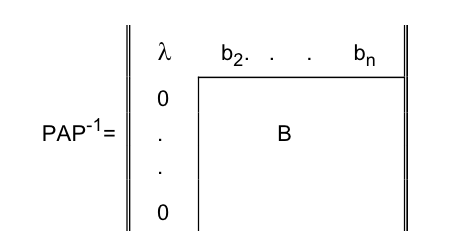
\includegraphics[width=0.4\textwidth]{imgs/img06.png}
\end{center}

%% TO REVIEW FROM HERE
\section{Riduzione di una matrice hermitiana in forma
tridiagonale: il metodo di Householder}
Il metodo delle potenze \`e adatto per matrici sparse e se
si vogliono solamente pochi autovalori. \\
Nel caso si vogliano ottenere tutti, o quasi tutti, gli autovalori
\begin{enumerate}
\item si trasforma $A$ in una forma $B$ più condensata (cioè con più
  zeri) \emph{simile}
\item si calcolano gli autovalori di $B$ con un procedimento iterativo
\end{enumerate}

\subsection{Trasformazioni}
Forma condensate:
\begin{itemize}
\item \emph{Hessemberg} (\ref{def:hessemberg})
  $ a_{ij} = 0$ per $i > j+1$
  $$
  H_n = \begin{bmatrix}
    h_{1,1} & h_{1,2} & h_{1,3} & \cdots    & h_{1,n} \\
    h_{2,1} & h_{2,2} & h_{2,3} & \cdots    & h_{2,n} \\
    0       & h_{3,2} & h_{3,3} & \cdots    & h_{3,n} \\
    \vdots  & \ddots  & \ddots  & \ddots    & \vdots  \\
    0       & \cdots  & 0       & h_{n,n-1} & h_{n,n}
  \end{bmatrix}
  $$
Quest è la forma ottenuta nel caso più generale.

\item Tridiagonale
  $$
  T_n = \begin{bmatrix}
    t_{1,1} & t_{1,2} & 0 & \cdots  & 0 \\
    t_{2,1} & t_{2,2} & t_{2,3} & \ddots  & \vdots  \\
    0       & t_{3,2} & t_{3,3} & \ddots  & 0 \\
    \vdots  & \ddots  & \ddots  & \ddots  & t_{n-1,n}  \\
    0       & \cdots  & 0     & t_{n,n-1} & t_{n,n}
  \end{bmatrix}
  $$
Se la matrice $A$ è hermitiana, e la trasformazione viene eseguita con
matrici unitarie (Householder), la matrice $B$ risulta hermitiana e
tridiagonale (rientra in Hessemberg).
\end{itemize}

\section{Il metodo di Householder}
La trasformazione per similitudine unitarie della matrice $A$ nella matrice $B$
\`e fatta per passi successivi
\begin{equation}
  %% (16)
  \label{eq:09}
  A^{(k+1)} = T^{-1}_k A^{(k)} T_k,\;  k = 1, 2, \ldots , m-1
\end{equation}
dove
$$ A^{(1)}=A \quad \text{e} \quad A^{(m)}=B$$
per cui, posto $T = T_1 T_2 \ldots T_{m-1}$, risulta $B = T^{-1} AT$,
e se $x$ \`e autovettore  di $B$, $T x$ \`e autovettore di $A$.
\\ \\
Sia $A \in \mathbb{C}^{n \times n}$ una matrice hermitiana;
si considerino le trasformazioni (\ref{eq:09}), con $m = n-1$,
in cui le matrici $T_k$ siano matrici elementari di Householder
(hermitiane e unitarie):
$$T_k= I − \beta_k u_k u_k^{H} ,$$

costruite in modo che nella matrice $T_k A^{(k)}$ siano nulli tutti gli
elementi della $k$-esima colonna, con l'indice di riga maggiore di $k + 1$.
Al primo passo, posto

$$
A^{(1)} = A =
\left[
\begin{array}{llll}
a_{11}^{(1)} &  &              & a_1^{H}           \\
             &  &              &                   \\
a_1          &  &              & B^{(1)}
\end{array}
\right]
\begin{array}{l}
\} 1 \text{ riga}                                  \\
                                                   \\
\} n-1 \text{ righe}
\end{array}
$$
si consideri la matrice elementare di Householder $P^{(1)} \in
 \mathbb{C}^{(n-1) \times (n-1)}$ tale che
$$ P^{(1)}a_1 = \alpha_1 e_1$$
dove $e_1$ \`e il primo vettore della base canonica di $\mathbb{C}^{n-1}$.
 La matrice
$$
T_1 =
\left[
\begin{array}{llll}
  1          &  &              & 0^{H}             \\
             &  &              &                   \\
  0          &  &              & P^{(1)}
\end{array}
\right]
$$
\`e tale che nella matrice
$$
A^{(2)} = T_1^{-1}A^{(1)}T_1 = T_1 A^{(1)} T_1
$$
sono nulli tutti gli elementi della prima colonna con indice di riga maggiore
di due e dei simmetrici elementi della prima riga. \\
Al $k$-esimo passo la sottomatrice principale di testa di ordine $k + 1$ di
$A^{(k)}$ risulta tridiagonale hermitiana e $A^{(k)}$ ha la forma
$$
A^{(k)} =
\left[
\begin{array}{ccccc}
  C^{k}      &  & b_k          &  & O              \\
             &  &              &  &                \\
  b_k^{H}    &  & a_{kk}^{(k)} &  & a_k^{H}        \\
             &  &              &  &                \\
  O          &  & a_k          &  & B^{(k)}
\end{array}
\right]
\begin{array}{l}
\} k-1 \text{ righe}                               \\
                                                   \\
\} 1 \text{ riga}                                  \\
                                                   \\
n-k \text{ righe}
\end{array}
$$
dove $C^{(k)} \in \mathbb{C}^{(k-1) \times (k-1)}$ \`e tridiagonale hermitiana e
$b_k \in  \mathbb{C}^{k-1}$ ha nulle le
prime $k-2$ componenti. Sia $P^{(k)} \in \mathbb{C}^{(n-k) \times (n-k)}$
la matrice di Householder tale che
$$P^{(k)} a_k = \alpha_k e_1$$
dove $e_1$ \`e il primo vettore della base canonica di $C_{n-k}$ .
Posto
$$
T_k =
\left[
\begin{array}{llll}
I_k & & & 0^{H}                                    \\
 & & &                                             \\
0  & & & P^{(k)}
\end{array}
\right]
$$

risulta

$$A^{(k+1)} = T_k^{-1} A^{(k)} T_k = TkA^{(k)} Tk =
\left[
\begin{array}{ccccc}
  C^{k}   &  & b_k          &  & O              \\
          &  &              &  &                \\
  b_k^{H} &  & a_{kk}^{(k)} &  & a_k^{H}P^{(k)} \\
          &  &              &  &                \\
  O       &  & P^{(k)}a_k   &  & P^{(k)}B^{(k)} P^{(k)}
\end{array}
\right]
$$

Poich\'e il vettore $P^{(k)} a_k \in \mathbb{C}^{n−k}$ ha nulle le
componenti di indice maggiore o uguale a due, la sottomatrice
principale di testa di ordine $k+2$ della matrice $A^{(k+1)}$ \`e
tridiagonale hermitiana. Applicando il procedimento $n - 2$ volte si
ottiene la matrice $B = A^{(n−1)}$ tridiagonale hermitiana.

Se $A$ non è hermitiana si ottiene la forma di Hessemberg.
\begin{figure}[h]
 \centering
 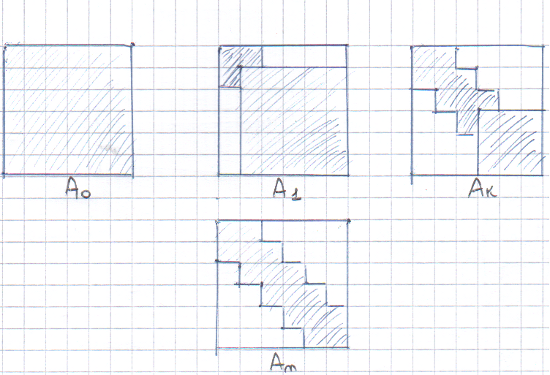
\includegraphics{./imgs/tridiagonal.png}
 % tridiagonal.png: 550x375 pixel, 150dpi, 9.31x6.35 cm, bb=0 0 264 180
 \caption{Passi della trasformazione di una matrice in forma tridiagonale}
\end{figure}


\begin{notes}
  Nel libro esattamente in questo punto vengono fatti dei conti per
  stabilire i costi delle varie operazione, che ometto in quanto il
  Bevilacqua non li ha nominati a lezione.
\end{notes}

La trasformazione $A^{(k)} \rightarrow A^{(k+1)}$ richiede solo $2(n -
k)^2$ operazioni moltiplicative. Il metodo di Householder per
tridiagonalizzare una matrice hermitiana richiede dunque
$$
\displaystyle \sum_{k-1}^{n-2} 2(n-k)^{2} \approx \frac{2}{3}n^{3}
\quad \text{operazioni moltiplicative}
$$

\begin{workinprogress}
  Per chi ne ha voglia: aggiungere disegnini fatti a lezione
\end{workinprogress}
%% Parte presa a lezione
\begin{comment}
da $A$ e $B$ di Hesemberg con opportune con trasformazioni
di Hessemberg
$$ P = I - \beta \mu \mu^{H}$$
$P$ Hermitiana unitaria \\
$\beta$ e $\mu$ scelti in modo che sia
$ P_x = \alpha e_1$ per un dato $x$
(Copiare vari disegnini)
$|\alpha| = ||x||_2$ \\
$A$ Hermitiana
Disegnino 6 x 6
\\
Prendiamo $P_{n-1}$ tale che
$$ P_{n-1} x = \alpha e_1$$
Allunghiamo la matrice $P_{n-1}$

Se $A$ \`e hermitiana alloa
$QAQ^{H}$ \`e Hermitiana

Complessiata $O(\frac{2}/{3}n^{3})$

Discorso della Diade
$P=I - \beta \mu \mu^{H}$
$$ PA = A - \beta \mu \mu^{H} $$

Diciamo specifico nel caso Hermitiano:
Triagonale hermitiana \\
$B_n$ tridiagonale hermitiana
Copiare maledetto disegnino \\
Ipotesi $B_n$ irriducibile: nel caso tridiagonale implica
tutti i $\beta_i \neq 0$ (L'analisi del grafo \`e OK).
Non pu\`o avere autovalori multipli (algebrica = gemetrica) \\
Se avesse $\lambda$ con molteplicita 2 allora
$rank(B_n - \lambda I) = n-2$  non esisterebbe nessuna
sottomatrice quadrata di $B_n -\lambda I$ con rango $n-1$
\\
Assurdo!!
\\
\\
Propriet\`a dei minori principali (di testa) di $B_n$\\
blabla
Successioni importanti blablabla successioni di Sturm
che permettono di separare gli zeri di tutti
\end{comment}

\begin{workinprogress}
Qua il Bevilacqua ha fatto una digressione sulle propriet\`a
dei minori principali di testa... per chi ha voglia, li metta.
\end{workinprogress}

%% 3 Maggio
\section{ Calcolo degli autovalori delle matrici tridiagonali
  hermitiane con la successione di Sturm}
Per calcolare gli autovalori di una matrice tridiagonale hermitiana
conviene utilizzare metodi iterativi che facciano ricorso al
polinomio caratteristico solo se il numero degli autovalori che si
vogliono determinare \`e piccolo rispetto alle dimensioni della
matrice. 

Riassumiamo i passi del metodo:
\begin{itemize}
\item utilizziamo lo sviluppo di Laplace per calcolare il polinomio
  caratteristico della matrice
\item la particolare struttura della matrice ci permette di calcolare
  lo sviluppo in modo iterativo ed efficiente
\item utilizziamo il metodo di Newton per calcolare gli zeri del
  polinomio caratteristico
\item per sapere in che intervallo lanciare la ricerca degli zeri
  usiamo il teorema di Sturm che sfrutta il numero di inversioni di segno
\end{itemize}

Sia $B_n \in \mathbb{C}^{n \times n}$ la matrice tridiagonale
hermitiana definita da
$$
B_n =
\left[
  \begin{array}{ccccc}
    \alpha_1 & \overline{\beta}_2 &        &         &                    \\
    \beta_2  & \alpha_2           & \ddots &         &                    \\
             & \ddots             & \ddots & \ddots  &                    \\
             &                    & \ddots & \ddots  & \overline{\beta}_n \\
             &                    &        & \beta_n & \alpha_n           \\
  \end{array}
\right]
\/
$$

Se la matrice $B_n$ \`e riducibile, cio\`e se esiste
almeno un indice $j, 2 \leq j \leq n$, tale che $\beta_j = 0$, allora
il problema del calcolo degli autovalori di $B_n$ \`e ricondotto al
calcolo degli autovalori di due matrici di ordine inferiore. Infatti
si ha
$$
B_n =
\left[
  \begin{array}{llll}
    C_{j-1} &  &  & O \\
            &  &  &   \\
    O       &  &  & D_{n-j+1}
  \end{array}
\right]
$$

in cui $C_{j−1} \in \mathbb{C}^{(j-1)\times(j-1)} , D_{n-j+1} \in
\mathbb{C}^{(n-j+1)×(n−j+1)}$ e quindi
$$ det(B_n - \lambda I) = det(C_{j-1} - \lambda I_{j-1})\;
det(D_{n-j+1} - \lambda I_{n-j+1}). $$

Se le matrici $C_{j−1}$ e $D_{n−j+1}$ sono a loro volta riducibili, si procede in modo analogo.

Si consideri perci\`o il caso che $B_n$ sia irriducibile e il suo
polinomio caratteristico, calcolato tramite lo sviluppo di Laplace
(\ref{sviluppo-laplace}) rispetto all'ultima riga, risulti
$$ P_n (\lambda) = det(B_n − \lambda I) = (\alpha_n -\lambda)
   P_{n-1}(\lambda) - |\beta_n|^2 P_{n-2} (\lambda) $$ 

con $P_i(\lambda)$ il polinomio caratteristico del minore principale
di testa di ordine $i$. Questo si può fare per ogni $i$
\begin{equation}
  %(21)
  \label{eigenvalues:10}
  \begin{array}{l}
    P_0(\lambda) = 1               \\
    P_1(\lambda) = \alpha_1 - \lambda \\
    P_i(\lambda) = (\alpha_i - \lambda)P_{i-1}(\lambda)
    - |\beta_i|^{2}P_{i-2}(\lambda) \quad i=2,3,\ldots
  \end{array}
\end{equation}
Quindi \`e possibile calcolare il valore che il polinomio $P_n
(\lambda)$ assume in un punto con $2(n - 1)$ moltiplicazioni
(supponendo di aver gi\`a calcolato $|\beta_i|^2$, $i = 2, 3,\ldots, n$).

Gli autovalori di $B_n$ vengono quindi calcolati risolvendo
l'equazione caratteristica
\begin{equation}
  % (23)
  \label{eigenvalues:11}
  P_n(\lambda) = 0
\end{equation}
con un metodo iterativo. Se si utilizza il metodo di Newton, il
calcolo di $P_n (\lambda)$ pu\`o essere fatto con le seguenti
relazioni ricorrenti, ottenute derivando rispetto a $\lambda$ entrambi
i membri delle (\ref{eigenvalues:10}):
$$
\begin{array}{l}
  P_0'(\lambda) = 0 \\
  P_1'(\lambda) = -1 \\
  P_i'(\lambda) = (\alpha_i − \lambda)P_{i-1}' (\lambda) -
  P_{i-1} (\lambda) − |\beta_i|^2 P_{i-2}'(\lambda),
  \quad i = 2, 3, \ldots, n.
\end{array}
$$

La formula di aggiornamento del metodo di Newton diventa quindi
$$ x_{i+1} = x_i - \dfrac{P_n(x_i)}{P'_n(x_i)}$$

Quindi il rapporto $P_n(\lambda)/P_n'(\lambda)$, che interviene ad
ogni passo del metodo di Newton, pu\`o essere calcolato con $4(n − 1)$
moltiplicazioni e una divisione.

Per separare le radici di (\ref{eigenvalues:11}) conviene sfruttare le
propriet\`a delle successioni di Sturm. Infatti nel seguente teorema
si dimostra che i polinomi $P_i(\lambda)$ formano una successione di
Sturm.

\begin{theo}
\label{eigenvalues:12}
Sia $A \in \mathbb{C}^{n \times n}$  hermitiana, e sia $A^k$ la
sottomatrice principale di testa di ordine $k$ di $A$.
Allora gli autovalori di $A_k$ separano gli autovalori di $A_{k+1}$ ,
per $k = 1, \ldots, n - 1$.
\end{theo}


\begin{theo}
\label{eigenvalues:13}
Se $\beta_i \neq 0$, per $i = 2, 3, \ldots , n$,
 la successione dei polinomi
$P_i (\lambda), i = 0, 1, \ldots, n$ verifica le seguenti propriet\`a:
\begin{enumerate}
\item  $P_0 (\lambda)$ non cambia segno;
\item se $P_i (\lambda) = 0$, allora $P_{i−1}(\lambda)P_{i+1}
(\lambda) < 0$, per $i = 1, 2, \ldots, n - 1$
\item se $P_n(\lambda) = 0$, allora $P'_n(\lambda)P_{n−1} (\lambda) < 0$
 (e quindi $P_n (\lambda)$ ha tutti zeri di molteplicit\`a 1).

\end{enumerate}
Una successione di polinomi che verifica le propriet\`a
1), 2) e 3) \`e detta successione di Sturm.
\end{theo}
\begin{thproof}
 La 1) \`e ovvia. Per la 2), si osservi che da
(\ref{eigenvalues:10}) si ha $P_{i−1} (\lambda)P_{i+1}(\lambda) \leq 0$.
Ma se fosse $P_{i−1} (\lambda)P_{i+1} (\lambda) = 0 $ e $P_i (\lambda)
= 0$, allora sarebbe $P_{i−1} (\lambda) = P_{i+1} (\lambda) = 0$, da
cui, per ricorrenza, seguirebbe $P_0 (\lambda) = 0$, che \`e assurdo.
Da ci\`o segue anche che gli zeri $\lambda_j^{(n)} , j = 1, 2, \ldots , n$,
 di $P_n (\lambda)$ sono distinti dagli zeri
$\lambda_j^{(n-1)}, j = 1, 2, \ldots , n - 1$, di $P_{n−1} (\lambda)$ e quindi,
 per il teorema (\ref{eigenvalues:12}), gli zeri $\lambda_j^{(n-1)}$ separano
strettamente gli zeri $\lambda_j^{(n)}$ , cio\`e
$$
\lambda_{j+1}^{(n)} < \lambda_{j}^{(n-1)} < \lambda_{j}^{(n)},
j=1,2,\ldots,n-1
$$

Da questo fatto, tenendo presente che il coefficiente di
$\lambda^i$ in $P_i(\lambda)$ \`e $(−1)^i$ ,
e quindi $\displaystyle \lim_{\lambda \to - \infty}P_i(\lambda) = +\infty$,
segue la 3).
\begin{center}
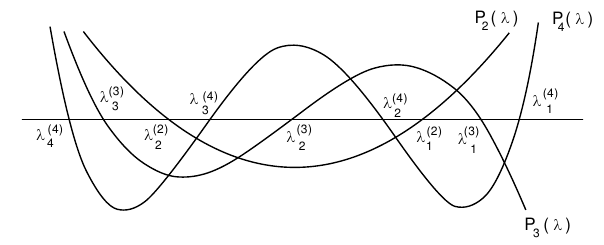
\includegraphics[width=0.7\textwidth]{imgs/grafico01.png}
\end{center}
\end{thproof}

\begin{theo}[Sturm]
Se $\{P_i (\lambda)\}, i = 0, 1, . . . , n,$  una successione di Sturm,
il numero $w(b) − w(a)$ \`e uguale al numero di zeri di $P_n (\lambda)$
 appartenenti all’intervallo $[a, b)$.
\end{theo}

\begin{thproof}
 Si faccia variare $\lambda$ con continuit\`a da $a$ verso $b$.
Si pu\`o avere una variazione nel numero $w(\lambda)$ solo quando
$\lambda$ incontra uno zero di uno dei
polinomi $P_i (\lambda)$.
Si consideri perci\`o un $\lambda^∗$ tale che $P_i (\lambda^∗ ) = 0$
 per un indice $i$. \\
 Per la propriet\`a 1) del teorema (\ref{eigenvalues:13}) deve essere $i \neq 0$.
Si distinguono allora i due casi:
\begin{enumerate}
\item $i\neq n$ \\
In questo caso, per la propriet\`a 2) del teorema
(\ref{eigenvalues:13})  si ha
$$P_{i−1} (\lambda^∗ )P_{i+1} (\lambda^∗ ) < 0.$$
Esiste perci\`o un numero $h$ tale che nell’intervallo
$[\lambda^∗ − h, \lambda^∗ + h]$
\`e ancora
$$P_{i−1} (\lambda)P_{i+1} (\lambda) < 0$$
e
$$
P_i(\lambda) \neq 0
$$

 eccetto che nel punto $\lambda^∗$ . Poich\'e per ogni
 $\lambda \in [\lambda^∗ − h, \lambda^∗ + h]$ i due
  polinomi $P_{i−1} (\lambda)$ e $P_{i+1} (\lambda)$
  hanno segno discorde, $P_i(\lambda)$ deve avere in
 questo intervallo segno concorde con uno dei due e discorde con
l’altro.
Quindi nella sequenza $P_{i−1} (\lambda), P_i (\lambda), P_{i+1} (\lambda)$
 vi \`e una sola variazione
 di segno in tutto l’intervallo $[\lambda − h, \lambda + h]$
, cio\`e il fatto che $P_i (\lambda)$ si
 annulli in $\lambda^∗$ non comporta variazioni del numero
$w(\lambda)$.

\item $i = n$\\
 In questo caso, poich\`e per la propriet\`a 3) del teorema (\ref{eigenvalues:13}) il
 polinomio $P_n(\lambda)$ ha radici semplici,
la sua derivata $P_n' (\lambda)$ non si annulla
in $\lambda^∗$ ed esiste un numero $h$ tale che nell’intervallo
$[\lambda^∗ -h, \lambda^∗ +h] \; P_n (\lambda)$
 ha lo stesso segno che $P_n (\lambda)$ ha in
$\lambda^∗ + h$ e segno opposto a quello che
 $P_n (\lambda)$ ha in $\lambda^∗ - h$.
Se $h$ tale che nell’intervallo $[\lambda^∗ − h, \lambda^∗ + h]$
 anche
 $P_{n−1} (\lambda)$ non si annulla, poich\'e per la propriet\`a 3)
 del teorema (\ref{eigenvalues:13})
 $P_{n−1} (\lambda)$ ha segno opposto a quello di
$P_n (\lambda)$ per $\lambda \in [\lambda^∗ − h, \lambda^∗ + h]$,
 la  sequenza $P_{n−1} (\lambda^∗ + h), P_n (\lambda^∗ + h)$
 presenta una variazione di segno,
 mentre la sequenza $P_{n−1} (\lambda^∗ - h), P_n (\lambda^∗ - h)$
 non presenta alcuna variazione di segno.
\end{enumerate}
Se ne conclude che il numero di variazioni di segno in tutta la
sequenza $P_0 (\lambda), P_1 (\lambda), \ldots , P_n (\lambda)$ pu\`o
cambiare solo nei punti in cui si annulla $P_n (\lambda)$, ed
esattamente aumenta di $1$ ogni volta che si annulla $P_n (\lambda)$.
Nella tesi del teorema l’intervallo $[a, b)$ \`e aperto a destra
perch\'e se fosse

$P_n (b) = 0$, poich\'e $P_n(b)$ viene assegnato lo stesso segno
assunto in $b$ da $P_{n−1} (\lambda)$, che diverso da zero in un
intorno sinistro di $b$, $w(\lambda)$ non cambia in tale
intorno. Perci\`o la radice $b$ non altera il numero di variazioni di
segno.
\end{thproof}
%%Risultato serve a metodo di bisezione
%$$p_n(a) \cdot p_n(b) < 0$$
%$V(b) - V(a)$ \\

%% Appunti presi a lezione
\begin{comment}
Propriet\`a dei polinomi caratteristici dei minori principali
di testa di una matrice tridiagonale Hermitiana, $B$
%% Disegnino
$$
p_n(\lambda) = (\alpha_n - \lambda)p_{n-1}(\lambda) -
| \beta_n|^{2} p_{n-2}(\lambda)
$$

$$
p_i(\lambda) = (\alpha_i - \lambda)p_{i-1}(\lambda) -
|\beta_i|^{2}_{i-2}(\lambda) \quad i=n,\ldots, 1, 0
$$
$$ p_0(\lambda)=1 \quad p_2(\lambda) = (\alpha_2 -\lambda)(\alpha_1-\lambda)
 - |\beta_2|^{2} \cdot 1
$$
Si pu\`o calcolare la derivata..
$$
p_i'(\lambda) = - \alpha_i p_{i-1}'(\lambda) +
 (\alpha_i - \lambda)p_{i-1}'(\lambda) - |\beta_i|^{2} p_{i-2}(\lambda)
$$
Metodo di newton
$$
x_{i+1} = x_i - \dfrac{p_n(x_i)}{p_n'(x_i)}
$$
\`e una successione di Sturm: sevono per separare gli zeri

\begin{defn}[Successione di sturm]
$$
\{ p_0(\lambda), p_1(\lambda), \ldots, p_n(\lambda) \}
$$

\begin{enumerate}
\item $p_0(\lambda) \neq 0$ ( per ogni $\lambda$)
 \item se $p_i(\lambda)=0 \quad 1 \leq i \leq n-1$ allora
   $p_{i-1}(\lambda) p_{i+1}(x) < 0 $
 \item Se $p_n(\lambda)=$ allora $p_n'(\lambda)p_{n-1}(\lambda) < 0 $
\end{enumerate}
\end{defn}
Matrice irriducibile, quindi $\beta_i \neq 0$
Se $p_i(\lambda) =det(B_i - \lambda I)$
la successione $\{p_0, \ldots, p_n \}$ \`e di Sturm. Infatti

\begin{enumerate}
\item $p_0(\lambda) = 1 \neq 0$
 \item $p_{i+1} (\lambda) = \cancel{(\alpha_{i+1} - \lambda)p_{i}(\lambda)}_{=0} -
 \underbracket{| \beta_{i+1}|^{2}}_{\neq 0 }p_{i-1}(\lambda)
$
%% Schema dei segni di p1 e p2

\item
% Altro schemino

\end{enumerate}
Sia $V(\lambda)$ il numero delle variazioni di segno nell'insieme
ordinato $\underbracket{p_0(\lambda)}_{+},
\underbracket{p_1(\lambda)}_{-}, \ldots p_n(\lambda)$
$V(\lambda) = 4$ numero di variazioni di segno

\end{comment}



%% Bevilacqua 13 Maggio
\section{Metodo $QR$}
L'idea alla base del metodo $QR$ e di generare una successione di
matrici $A_1 \ldots A_k$ tutte simili ad $A$, ma con $A_k$ triangolare
superiore con gli autovalori sulla diagonale.\\
Il metodo può sfruttare diversi metodi di fattorizzazione, ma la
migliore risulta essere la $QR$ perch\'e
\begin{itemize}
\item esiste sempre
\item usa trasformazioni unitarie che sono pi\`u stabili
\end{itemize}

\subsection{Metodo $QR$ con trasformazioni di Householder}
Nel metodo $QR$ viene generata una successione $\{A_k \}$
di matrici nel modo seguente: posto
$$A_1 = A,$$
per $k = 1, 2, \ldots$, si calcola una fattorizzazione $QR$ di $A_k$
\begin{equation}
   % (26)
  \label{eigenvalues:14}
  A_k = Q_k R_k
\end{equation}
dove $Q_k$ \`e unitaria e $R_k$ \`e triangolare superiore, e si
definisce la matrice $A_{k+1}$ per mezzo della relazione
\begin{equation}
  % (27)
  \label{eigenvalues:15}
  A_{k+1}= R_k Q_k
\end{equation}
Da (\ref{eigenvalues:14}) e (\ref{eigenvalues:15})  risulta che

\begin{equation}
   % (28)
  \label{eigenvalues:16}
A_{k+1} = Q_k^H A_k Q_k ,
\end{equation}
e quindi le matrici della successione $\{A_k \}$ sono tutte simili
fra di loro, infatti
$$ Q_{k} A_{k+1} Q_{k}^{H} = Q_{k} R_{k} \cancel{Q_{k} Q_{k}^{H}} = A_{k}$$

Sotto opportune ipotesi la successione converge ad una matrice
triangolare superiore (diagonale se $A$ \`e hermitiana) che ha
come elementi diagonali gli autovalori di $A$.\\
Il costo dell'algoritmo $QR$ \`e   $O(n^3)$.

\paragraph{Propriet\`a interessanti e miglioramento dell'efficienza}
\begin{itemize}
\item Se $A_k$ \`e Hermitiana, lo \`e anche $A_{k+1}$ \\
$$R_{k}^{-1} A_{k+1} R_{k} = \cancel{R_{k}^{-1} R_{k}} Q_{k} R_{k} = A_{k}$$
\item
Inoltre se la matrice precedente \`e di Hessemberg e si moltiplica
per  una triangolare a sinistra a destra, otteniamo una Hessemberg
$$ A_{k+1} = R_{k} A_{k} R_{k}^{-1} $$

\end{itemize}
Eseguiamo quindi una procedura di "bootstrap" con
$$ A \xrightarrow{\text{Householder}} \text{Hessemberg} $$
 questo \`e un bel vantaggio in termini di costi:  $O(n^{3})  \rightarrow O(n^{2})$. \\
Idem per il caso Hermitiano, in questo caso passiamo
a costo lineare $O(n)$


\subsection{Convergenza}
Per prima cosa, al fine di dimostrare la convergenza,
introduciamo il seguente risultato:
\begin{theo}
Se $A$ \`e non singolare e gli $r_{ii}$ della matrice $R$ sono reali e positivi,
allora le fattorizzazioni $Q$ e $R$ sono uniche.
  \end{theo}
  \begin{thproof}
$$  A = QR $$
Per prima cosa dimostriamo che data una qualsiasi
fattorizzazione $QR$, possiamo riportarci al caso
$Q_1R_1$ con $R_1$ avente $r_{ii}$ tutti positivi.
Introduciamo una matrice di fase:
$$A = QR = \underbracket{Q S^{H}}_{Q_1} \underbracket{S R}_{R_1}$$
Sia infatti
$$
R =
\begin{pmatrix}
  r_{11}  & r_{12} \\
 0 & r_{22}
\end{pmatrix}
\qquad
S
=\begin{pmatrix}
 \frac{|r_{11}|}{r_{11}} & 0 \\
 0 & \frac{|r_{12}|}{r_{22}}
\end{pmatrix}
$$
Allora

$$
R_1 =
\begin{pmatrix}
  |r_{11}|  & * \\
 0 & |r_{22}|
\end{pmatrix}
$$
Dimostriamo adesso l'unicit\`a di tale fattorizzazione:
per assurdo, siano le seguenti due diverse fattorizzazioni $QR$:
$$ QR = \hat{Q} \hat{R} \quad r_{ii}>0 \;,\; \hat{r_{ii}}> 0 $$
Ma allora, poich\`e:
\begin{enumerate}
\item il prodotto di matrici unitarie \`e una  matrice unitaria
 \item l'inversa di una triangolare superiore , se esiste,
   \`e ancora una triangolare superiore. Inoltre l'insieme
   delle triangolari superiori \`e chiuso rispetto al prodotto.
\end{enumerate}
Ottiniamo quindi:
$$ \underbracket{\hat{Q}{Q}}_{\text{unitaria}} =
\underbracket{\hat{R}R^{-1}}_{\text{t.sup}}
$$
Ma una matrice $V$ che sia unitaria e triangolare superiore
 deve essere necessariamente diagonale in quanto
$$
\underbracket{V^{H}}_{\text{t.inf}} =\underbracket{V^{-1}}_{\text{t.sup}}
 \rightarrow V \text{ diagonale}
$$
In sostanza stiamo lavorando quindi con una matrice
\emph{diagonale} e \emph{unitaria}. Sappiamo per\`o
\begin{enumerate}
\item $d_{ii} = \dfrac{\overbracket{\hat{r_{ii}}}^{>0}}
  {\underbracket{r_{ii}}_{>0}} > 0$
\item Essendo la matrice unitaria, affinche $D=D^{H} = D^{-1}$
  deve essere $d_{ii}=1$
\end{enumerate}
Concludiamo che deve essere
$$ \hat{R}R^{-1} = I \quad \Rightarrow \quad
\hat{R} = R \quad \Rightarrow \quad \hat{Q} = Q$$
% In questo caso inoltre
% queste due matrici devono essere diagonali, in quanto
% T.sup = t.inf
% \vspace{1cm}
% $$ \underbracket{\hat{R}}_{tsup}\underbracket{R^{-1}}_{tsup} = D \text{ unitaria} $$
% $$ d_{ii} \hat{r_{ii}}/ r_{ii}  > 0 $$
% Allordi $d_{ii} = 1$
% Quiindi $D = I$, matrice identica.
  \end{thproof}


%% A Lezione
 \begin{comment}
$$ A = A_1 = Q_1 R_1$$ \\
$$ A_2 = R_1Q_1 = Q_2 R_2$$
$$ A_{k+1} = R_{k} Q_{k} = Q_{k+1} R_{k+1} $$
Le matrice $A_k$ sono simili tra loro,
$$ Q_{k} A_{k+1} Q_{k}^{H} = Q_{k} R_{k} \cancel{Q_{k} Q_{k}^{H}} = A_{k}$$
\begin{itemize}
\item Se $A_k$ \`e Hermitiana, lo \`e anche $A_{k+1}$ \\
$$R_{k}^{-1} A_{k+1} R_{k} = \cancel{R_{k}^{-1} R_{k}} Q_{k} R_{k} = A_{k}$$
\item
Inoltre se la matrice precedente \`e di Hessemberg e si moltiplica
per  una triangolare a sinistra a destra, otteniamo una Hessemberg
$$ A_{k+1} = R_{k} A_{k} R_{k}^{-1} $$

\end{itemize}
C'e una procedura di "bootstrap" con
$$ A \xrightarrow{\text{Householder}} \text{Hessemberg} $$
 questo \`e un bel vantaggio $O(n^{3})  \rightarrow O(n^{2})$

Item per il discorso Hermitiano, in questo caso passiamo
a costo lineare $O(n)$


Rendiamo \emph{unica} la fattorizzazione $QR$:
vale il seguente risultato:

\begin{theo}
Se $A$ \`e non singolare e gli $r_ii $ di $R$ sono reali e
positivi, allora le fattorizzazioni $Q$ e $R$ sono uniche, perch\`e:
  \end{theo}
  \begin{thproof}
$$    A = QR $$
Introduciamo fra due fattorizzazioni una matrice di fase
$$A = QR = Q S^{H} S R$$
$SR$ = $R_1$
$QS^{H} = Q_1$
E ce ne \`e una sola: se ce ne fossero 2 per assurdo:
$$ QR = \hat{Q} \hat{R}$$
$$ r_{ii} > 0 \quad \hat{r_{ii}}$$
$$ \underbracket{\hat{Q}^{Q}}_{\text{unitaria}} =
\underbracket{\hat{R}R^{-1}}_{t.sup}
$$
In questo caso inoltre
queste due matrici devono essere diagonali, in quanto
T.sup = t.inf
\vspace{1cm}
$$ \underbracket{\hat{R}}_{tsup}\underbracket{R^{-1}}_{tsup} = D \text{ unitaria} $$
$$ d_{ii} \hat{r_{ii}}/ r_{ii}  > 0 $$
Allordi $d_{ii} = 1$
Quiindi $D = I$, matrice identica.
  \end{thproof}
\end{comment}
Adesso possiamo dimostrare il seguente teorema. Putroppo non \`e possibile
verificarne le ipotesi a priori.
\begin{theo}[Convergenza]
\begin{enumerate}
\item $$ | \lambda_1| > | \lambda_2 | > \ldots > | \lambda_n | > 0 $$
in questo caso la matrice \`e diagonalizzabile
\item
Indicata con $X$ la matrice degli autovettori di $A$, tale che
\begin{equation}
% (30)
 \label{eigenvalues:19}
A = XDX ^{-1}
\end{equation}
in cui $D$ \`e la matrice diagonale il cui $i$-esimo elemento principale \`e $\lambda_i$ ,
si supponga che la matrice $X^{-1}$ ammetta la fattorizzazione $LU$.
\end{enumerate}
 Allora
esistono delle matrici di fase $S_k$ tali che

\begin{equation}
% (31)
 \label{eigenvalues:20}
\lim_{k \to \infty} S_k^{H} R_k S_{k-1} = \lim_{k \to \infty} S_{k-1}^{H} A_k S_{k-1} =T
\end{equation}
e
$$\lim_{k \to \infty} S_{k-1}^{H} Q_k S_k = I$$
dove $T$ \`e triangolare superiore con gli elementi principali uguali a
$\lambda_1 , \lambda_2 , \ldots,  \lambda_n$ .
 Quindi gli elementi principali di $A_k$ tendono agli autovalori di $A$. Se $A$
\`e una matrice hermitiana, allora $T$ \`e diagonale.
\end{theo}
\begin{thproof}
Facciamo una semplificazione che sul libro non viene fatta,
quindi la dimostrazione \`e pi\`u semplice.
$$ A = QR = Q_{1} R_1$$
Le due fattorizzazioni possono differire per il prodotto
di una matrice di fase, questo significa che
$$ Q_1 = QS^{H}  \qquad R_1 = SR $$
Utilizziamo il teorema precedente, utilizzando il fatto
che la fattorizzazione sia unica. \\ \\

 Il teorema viene dimostrato confrontando due fattorizzazioni $QR$
della matrice $A_k$ ottenute in due modi diversi.
\begin{enumerate}
\item
 Una prima fattorizzazione \`e data dalla seguente relazione
\begin{equation}
 % 32
  \label{eigenvalues:17}
 A^k = \underbracket{H_k}_{\text{tipo Q}} \underbracket{U_k}_{\text{tipo R}} ,
\end{equation}
dove
$$H_k = Q_1 Q_2 \ldots Q_k$$
\`e una matrice unitaria e
$$U_k = R_k R_{k−1} \ldots R_1$$
$$A^{k} = \underbracket{Q_1 Q_2 \ldots Q_k}_{\text{tipo Q}}
 \underbracket{R_k R_{k-1} \ldots R_1}_{\text{tipo R}}$$
Per dimostrare la (\ref{eigenvalues:17}) si procede per induzione: \\ \\
\textbf{Caso} $k=1$
 $$A = A_1 = H_1 U_1$$
 ovvio
\\
\\
\textbf{Caso} $k>1$ \\
Supposta valida la (\ref{eigenvalues:17}), da
  (\ref{eigenvalues:15}) e   (\ref{eigenvalues:16}) si ottiene
$$Q_k A_{k+1} = A_k Q_k $$
da cui
\begin{equation}
 \label{eigenvalues:18}
Q_1 \ldots Q_{k-1} Q_k A_{k+1} = Q_1 \ldots Q_{k-1} A_k Q_k = \ldots = AQ_1 \ldots Q_{k-1}
 Q_k
\end{equation}
e quindi
$$
\begin{array}{ll}
H_{k+1} U_{k+1} & = Q1 \ldots Q_k Q_{k+1} R_{k+1} R_k \ldots R_1 \\
 &  = Q_1 \ldots Q_{k-1} Q_k A_{k+1} R_k R_{k-1} \ldots R_1 \\
 & = AQ_1 \ldots Q_{k-1} Q_k R_k R_{k-1} \ldots R_1 = AH_k U_k = A_{k+1} ,
\end{array}
$$
cio\`e
 $A_{k+1} = H_{k+1} U_{k+1} $.

\item
Una seconda fattorizzazione $QR$ della matrice $A_k$ viene ottenuta dalla
relazione  (\ref{eigenvalues:19}).
Sia $X^{-1} = LU $ la fattorizzazione $LU$ di $X^{-1}$
 . Allora
$$A^k = XD^k X^{-1} = XD^k LU = XD^k LD^{-k} D^{k} U$$
Poich\`e gli elementi della matrice $D^k LD^{-k}$ sono dati da

\begin{equation}
 %34
\label{eigenvalues:20}
  \left\{
 \begin{array}{ll}
  l_{ij}\left(\dfrac{\lambda_i}{\lambda_j} \right)^{k} & \text{ per } i > j, \\
  1 & \text{ per } i =j \\
  0 & \text{ per } i < j
 \end{array}
 \right.
\end{equation}
e $|\lambda_i | < |\lambda_j | \;$ per $i > j$, si pu\`o porre

$$D^k LD^{-k} = I + E_k,$$
dove

$$\lim_{k \to \infty} E_k = 0$$
e quindi \`e
$$A^k = X(I + E_k )D^k U.$$
Indicata con
$$X = QR$$
una fattorizzazione $QR$ della matrice $X$, si ha

$$A^k = QR(I + E_k )D^k U = Q(I + RE_k R^{-1} )RD^k U,$$
e indicata con

\begin{equation}
\label{eigenvalues:21}
I + RE_k R^{-1} = P_k T_k
\end{equation}
una fattorizzazione $QR$ della matrice $I + RE_k R^{-1}$ si ha
\begin{equation}
%(36)
\label{eigenvalues:22}
A_k = (QP_k ) (T_k RD^k U ).
\end{equation}
La (\ref{eigenvalues:22}) da una seconda fattorizzazione $QR$ di $A_k$ :
infatti $QP_k$ \`e unitaria e $T_k RD^{k} U$ \`e triangolare superiore.
\end{enumerate}
Abbiamo due uguaglianze
\begin{openquestion}
qui si sta usando il teorema enunciato e dimostrato prima, ma perch\`e
lo pu\`o usare? Non mi \`e assolutamente chiaro. Dov\`e l'ipotesi che
i $r_{ii}$ sono reali? Quest'ultima parte \`e assolutamente da rivedere.
\end{openquestion}


$$ QP_k = Q_1 Q_2 \ldots Q_k$$
$$ T_kRD^{k} U = R_{k} \underbracket{R_{k-1} \ldots R_1}_{T_{k-1} RD^{k-1}U} $$
Ottieniamo
$$ QP_{k}= QP_{k-1} Q_k$$
$$ T_k RD^{k} U  = R_{k} T_{k-1} RD^{k-1} U$$
$$ Q_k = P_{k-1}^{H} P_k$$
$$ R_{k} = T_k R \cancel{D^{k}} D^{1\cancel{-k}} R^{-1} T^{-1}_{k-1}$$
Ricordiamo che
$$ (D^{k-1})^{-1}= D^{1-k}$$
\\
$$ A_k = Q_k R_k =
 \underbracket{P^{H}_{k-1}}_{\to \infty I}
\underbracket{P_{k}}_{\to \infty I}
\underbracket{ T_{k}}_{\to \infty I} RDR^{-1}
\underbracket{ T_{k-1}^{-1}}_{\to \infty I}
$$
\end{thproof}
\subsection{Indebolimento delle condizioni del teorema}
Le condizioni del teorema possono essere indebolite, infatti
\begin{enumerate}
\item Esistono
$$\lambda_i, \lambda_j, i \neq j,
 | \lambda_i| = | \lambda_j | =
\left\{
 \begin{array}{ll}
(a) &  \lambda_i = \lambda_j  (multipli) \\
(b) & \lambda_i \neq \lambda_j
 \end{array}
\right.
$$
nel caso (a) c'e' convergenza,
nel caso (b), convergenza a $T$ triangolare superiore a blocchi

\item
 Davamo per scontata la diagonalizzabilit\`a,
 supponiamo che non ci sia: c'e' lo stesso la convergenza.
\item

 $ X^{-1}$ non ha fattorizzazione LU, ma non c'e' convergenza
 \emph{ordinata}, autovalori non ordinati.
\end{enumerate}
\subsection{Tecnica di translazione: QR con shift}
La velocit\`a di convergenza del metodo $QR$ dipende per la (\ref{eigenvalues:20})
 dai rapporti
$|\lambda_i /\lambda_j |$ per $i > j$, e quindi per l’ipotesi
$$|\lambda_1 | > |\lambda_2 | > . . . > |\lambda_n | > 0$$
 dal numero
\begin{equation}
%(38)
\label{eigenvalues:23}
 \max_{1 \leq i \leq n-1}
\left|\dfrac{\lambda_{i+1}}{\lambda_i} \right|
\end{equation}
Se tale rapporto \`e vicino ad 1, la convergenza pu\`o essere lenta. In questo
caso per accelerare la convergenza si utilizza una tecnica di traslazione dello
spettro degli autovalori di $A$, detta di \emph{shift}.
Sia $\mu$ un numero che approssima un autovalore $\lambda$ meglio degli altri
autovalori. Le matrici $Q_k$ e $R_k$ , generate dal metodo $QR$ a partire dalla
matrice $A − \mu I$ possono essere costruite anche per mezzo delle seguenti
relazioni (metodo $QR$ con shift)

$$
\left.
\begin{array}{l}
 A_k - \mu I = Q_k R_k \\
A_{k+1} = R_k Q_k + \mu I
\end{array}
\right\}
\text{per } k=1,2, \ldots
$$

e risulta
$$Q_k A_{k+1} = A_k Q_k − \mu Q_k + \mu Q_k = A_k Q_k $$
Tenendo presente che gli autovalori di $A − \mu I$ sono $\lambda_i − \mu$ e che
 la velocit\`a
di convergenza \`e regolata dalla (\ref{eigenvalues:23}), \`e
 possibile scegliere un parametro $\mu$
in modo da accelerare la convergenza del metodo $QR$ con shift. \`E conveniente
scegliere per $\mu$ un valore che approssima $\lambda_n$ . Ci\`o pu\`o essere ottenuto
applicando il metodo $QR$ inizialmente senza shift per un certo numero $p$ di
iterazioni, e scegliendo $\mu = a_{nn}^{(p)}$ per le successive iterazioni con shift.
Poich\`e $\mu$ pu\`o essere modificato ad ogni iterazione \`e pi\`u conveniente
scegliere
\begin{equation}
 %(39)
\label{eigenvalues:24}
\mu_k = a_{nn}^{(k)} \quad k = 1, 2, \ldots
\end{equation}

Quando le condizioni di arresto verificata per $p = n−1$, si passa a operare sulla matrice
$B_k$ di ordine $n - 1$ ottenuta dalla matrice $A_k$ eliminando l'ultima riga e
l'ultima colonna. Per l'approssimazione degli altri autovalori si procede in
modo analogo.

%\subsection{Matrice di Sylvester}
%\begin{workinprogress}
% $$ S^{T}S - SS^{T} \neq 0$$
% non \`e normale, per risultato del condizionamento. \\
%Matlab, quando l'ordine della matrice cresce abbastanza,
%alcuni autovalori di $S$ calcolati con il metodo $QR$
%non hanno nessuna cifra significativa.
%Varianti del metodo $QR$ che vanno su sottoninsiemi
%degli autovalori dominanti in modulo
%\end{workinprogress}
%%%%%%%
% Commento perche' non e' presente nel programma
%
% Nic

%% Parte presa a lezione
\begin{comment}
\begin{theo}[Convergenza]
Ipotesi, non verificabili a priori \\
\begin{enumerate}
\item $$ | \lambda_1| > | \lambda_2 | > \ldots > | \lambda_n | > 0 $$,
in questo caso la matrice \`e diagonalizzabile
\item Se $X$ \`e la matrice degli autovettori cio\`e
$$ A  XDX^{-1}$$
esiste la fattorizzazione $X^{-1} = LU$
\end{enumerate}
 allora esistono matrici di fase $S_k$ tali che
$$ \lim_{k \to \infty} S_k^{H}R_{k} S_{k-1} = T $$
con $T$ triangolare superiore in cui
i $t_{ii} = \lambda_i $
\end{theo}
\begin{thproof}
Facciamo una semplificazione che sul libro non viene fatta,
quindi la dimostrazione \`e pi\`u semplice.
$$ A = QR = Q_{1} R_1$$
Le due fattorizzazioni possono differire per il prodotto
di una matrice di fase, questo significa che
$$ Q_1 = QS^{H}  \qquad R_1 = SR $$
Utilizziamo il teorema precedente, utilizzando il fatto
che la fattorizzazione sia unica. \\ \\

Due fattorizzazione $QR$ di $A^{k}$
\begin{enumerate}
\item $A^{k} = \underbracket{Q_1 Q_2 \ldots Q_k}_{\text{tipo Q}}
 \underbracket{R_1 R_2 \ldots R_k}_{\text{tipo R}}$ \\
 Dimostriamolo
$k=1$ \\
$$A= Q_{1} R_{1}$$
ovvio \\
$k=n$
$$ A^{k+1} = AA^{k} = AQ_1 W_2\ldots Q_k R_k \ldots R_1$$
$$AQ_1  \quad A_2 = Q_{1}^{H}A_1Q_1$$
$$ Q_1 A_2 = A_1 Q_1$$
\\
$$ A Q_1 Q_2 \ldots Q_k R_k \ldots R_1 = $$
$$ Q_1 A_2 Q_2 \ldots Q_k$$ =
$$ Q_1 Q_2 A_3 \ldots $$
=
$$ Q_1 \ldots Q_k A_{k+1} R_{k} \ldots R_1$$
=
$$ Q_1 \ldots Q_k Q_{k+1} R_{k+1} \ldots R_1$$
$$ Q_1 \ldots Q_k Q_{k+1} R_{k+1} \ldots R_1$$

\item
$$ A = XDX^{-1}$$
$$ A^{k}  XD^{k}X^{-1} = \underbracket{QR}_{X}D^{k}LU =$$
$$QRD^{k} L D^{-k} D^{k} U$$
(inseriamo D perch\`e esiste l'inversa)
$ D^{k} L D^{-k}$ \` triangolare inferore con 1 sulla diagonale
Nella pate inferiore
$$
\dfrac{\lambda_i^{k}}{\lambda_j^{k}}l_{j}
\rightarrow \left( \dfrac{\lambda_i}{\lambda_i} \right)^{k} l_{ij}
$$
Gli autovalori in modulo sono in modulo minore di 1, quindi
per $k \to \infty$ abbiamo convergenza verso la matrice
identica
$$ D^{K} L D^{-k} \xrightarrow {k \to \infty} I $$
$$ (I + E_{k}) \quad E_{k}\rightarrow 0$$

$$A^{k} = QR(I + E_k) R^{-1} RD^{k}U$$
=
$$ Q(I + \underbracket{RE_{k} R^{-1}}_{\rightarrow 0 }) R D^{k}U $$
=
$$ QP_k T_k RD^{k} U = QR$$

Allora abbiamo
$$ P_k \rightarrow I$$
$$ T_k \rightarrow I $$
Ottieniamo quindi
$$ A^{k}  \underbracket{QP_{k}}_{\text{tipo Q}}
\underbracket{T_k RD^{k}U}_{\text{tipo R}}
$$
$$QP_k  Q_1 Q_2 \ldots Q_k $$
$$ T_k R D^{k} U = R_{k}R_{k-1} \ldots R_1$$
Mancano un paio di passaggi e otteniamo la convergenza

$$ A_{k} \xrightarrow{k \to \infty}
T = RDR^{-1}
$$
\end{enumerate}
Abbiamo due uguaglianze
$$ QP_k = Q_1 Q_2 \ldots Qk$$
$$ Tk_RD^{k} U = R_{k} \underbracket{R_{k-1} \ldots R_1}_{T_{k-1} RD^{k-1U}} $$
Ottieniamo
$$ QP_{k}= QP_{k-1} Q_k$$
$$ T_k RD^{k} U  = R_{k} T_{k-1} RD^{k-1} U$$
$$ Q_k = P_{k-1}^{H} P_k$$
$$ R_{k} = T_k R \cancel{D^{k}} D^{1\cancel{-k}} R^{-1} T^{-1}_{k-1}$$
Ricordiamo che
$$ (D^{k-1})^{-1}= D^{1-k}$$
\\
$$ A_k = Q_k R_k =
 \underbracket{P^{H}_{k-1}}_{\to \infty I}
\underbracket{P_{k}}_{\to \infty I}
\underbracket{ T_{k}}_{\to \infty I} RDR^{-1}
\underbracket{ T_{k-1}^{-1}}_{\to \infty I}
$$
\end{thproof}
Le condizioni del teorema possono essere indebolite,
infatti
\begin{enumerate}
\item esistono
$$\lambda_i, \lambda_j, i \neq j,
 | \lambda_i| = | \lambda_j | =
\left\{
 \begin{array}{l}
(a)   \lambda_i = \lambda_j  (multipli) \\
(b)  \lambda_i \neq \lambda_j
 \end{array}
\right.
$$
nel caso (a) c'e' convergenza,
nel caso (b), convergenza a $T$ triangolare superiore a blocchi

\item
 Davamo per scontata la diagonalizzabilit\`a,
 supponiamo che non ci sia: c'e' lo stesso la convergenza.
\item

 $ X^{-1}$ non ha fattorizzazione LU, ma non c'e' convergenza
 \emph{ordinata}, autovalori non ordinati.
\end{enumerate}

Concetto di translate
$$ \underbracket{A}_{\lambda} \leftarrow \underbracket{A}_{\lambda}
- \underbracket{\alpha I}_{\alpha}
$$
$$ | \lambda_1 | > | \lambda_2 > | \lambda_3 |$$
$$ | \lambda - \alpha | > | \lambda_2 - \lambda| > |\lambda_3 - \alpha |$$
$\alpha$ t.c $|\lambda_n - \alpha$ piccolo
Questa si chiama $QR$ con SHIFT.
$$ \alpha = Q_{nn} $$
Quando la norma
$$ || Q^{(k)}_n, 1:n-1|| < \epsilon $$
$$\lambda_n \approx Q_{nn}^{(k)} $$
Buttiamo via
l'ultima riga e l'ultima colonna
ed eseguiamo la rifrazione
 \\
Matrice di Sylvester
$$ S^{T}S - SS^{T} \neq 0$$
 non \`e normale, per risultato del condizionamento. \\
Matlab, quando l'ordine della matrice cresce abbastanza,
alcuni autovalori di $S$ calcolati con il metodo $QR$
non hanno nessuna cifra significativa.

Varianti del metodo $QR$ che vanno su sottoninsiemi
degli autovalori dominanti in modulo
\end{comment}

\outbpdocument
